\documentclass[./memory.tex]{subfiles}

\begin{document}
\chapter{Implementation}
This chapter delves into the implementation of the frontend application,
building upon the architectural concepts discussed in the previous chapter. The
UI designs, which played a crucial role in determining a portion of the
application's structure, are also attached, as they helped compose the
application following Next.js principles.
\\[8pt]
The architectural concepts explained in the previous chapter are brought to life
through the practical implementation detailed here. By aligning the
implementation with the established architecture principles, a robust,
maintainable, and scalable application is ensured.
\\[8pt]
Moreover, we will explore the Next.js project structure, which provides a
framework for organizing components, pages, routing, and other features.
Understanding this expected structure is essential for maintaining consistency
and facilitating collaboration among developers.
\section{Designing the UI}
As explained in the planning chapter, the first task involved designing the UI.
The designs presented hereafter, were the initial implementation taking into
account the \emph{initial} objectives and requirements. Moreover, and explained
as well in the planning chapter, during the development of the dashboard page,
the team decided to change the model of the travel, improving it, and the
designs do not incorporate the changes made\footnote{The reason why designs were
	not updated, was due to lack of time, as being a single frontend I preferred not
	updating them, rather following the minimum styles and creating components
	accordingly. Needless to say that, in a corporation, the UI/UX team should
	update the designs according to the design system of such.}. Such changes
are visualized in the results chapter.
\\[8pt]
Given the absence of specific design requirements, the design was developed with
a set of self-defined requirements in mind. These requirements were:
user-friendly interface, reduced complexity to expedite component
implementation, an MVP (minimum viable product) approach, and focus on
mobile-first design principles.
\\
The primary objective was to create a user-friendly experience and UI that
prioritized ease of use and intuitive interactions. The design decisions were
influenced by my own experience in designing and working with user interfaces,
aiming to deliver a seamless and enjoyable user journey. However, it is worth
noting that predicting how users will interact with the application can be
challenging and prone to errors. Therefore, it is recommended to incorporate
internal tracking mechanisms to gain insights into user preferences and flows.
This tracking would enable product owners to better understand which features
and workflows users prefer, enhancing the application's usability. However, due
to the time constraints of an MVP development, implementing such tracking may
not be feasible.
\\
To ensure the development process met project timelines, the design aimed for
simplicity and efficiency, while ensuring an attractive user interface. By
minimizing the complexity in the design, the implementation of the components
became more streamlined and time-effective, enabling the team to focus on core
functionality and essential features. Nonetheless, and as explained in the
previous chapter, composition over inheritance will allow the developers to
update components without generating breaking changes to the current user
interface.
\\
In today's mobile-driven world, mobile-first principles are essential. With this
in mind, the design prioritized the mobile user experience, ensuring that the
application is optimized for mobile devices. By taking into account the unique
aspects of mobile devices, such as screen size and touch interactions, the
design focused on providing a seamless and intuitive experience for mobile
users. Needless to say, it would be more that interesting to perform a tracking
analysis on the usage of mobile versus non-mobile users of the application. The
results of such analysis would allow the design team to improve the application
for the specific platform, as well as knowing which platforms are more important
than others.
\\[8pt]
Finally, by adhering to these self-defined requirements, the design aimed to
strike a balance between user satisfaction, development efficiency, and the
delivery of a viable product. The section will delve deeper into the design
decisions made, explaining how these requirements influenced the design choices
and ultimately contributed to its creation.
\subsection{Authentication pages}
One of the requirements of the application is the possibility of authenticating
the user, in order to persist data accordingly. Allowing non-authenticated users
is not part of the MVP, but could be considered as a future feature.
\\[8pt]
The login and sign-up pages are very basic, simply requesting for the
information mandatory for each process to authenticate
\begin{enumerate}[label = -]
	\item\textbf{Login}. Requirements are user email and their password. The
	password must: include a lower and a capital letter, a number, a special
	symbol and be at least 8 characters long. These requirements have now
	become a common standard, and ensure protection over the user's account.
	\item\textbf{Sign-up}. Requirements are the same as login, with the addition
	of the first and last name, and a phone.
\end{enumerate}
\begin{figure}[H]
	\centering
	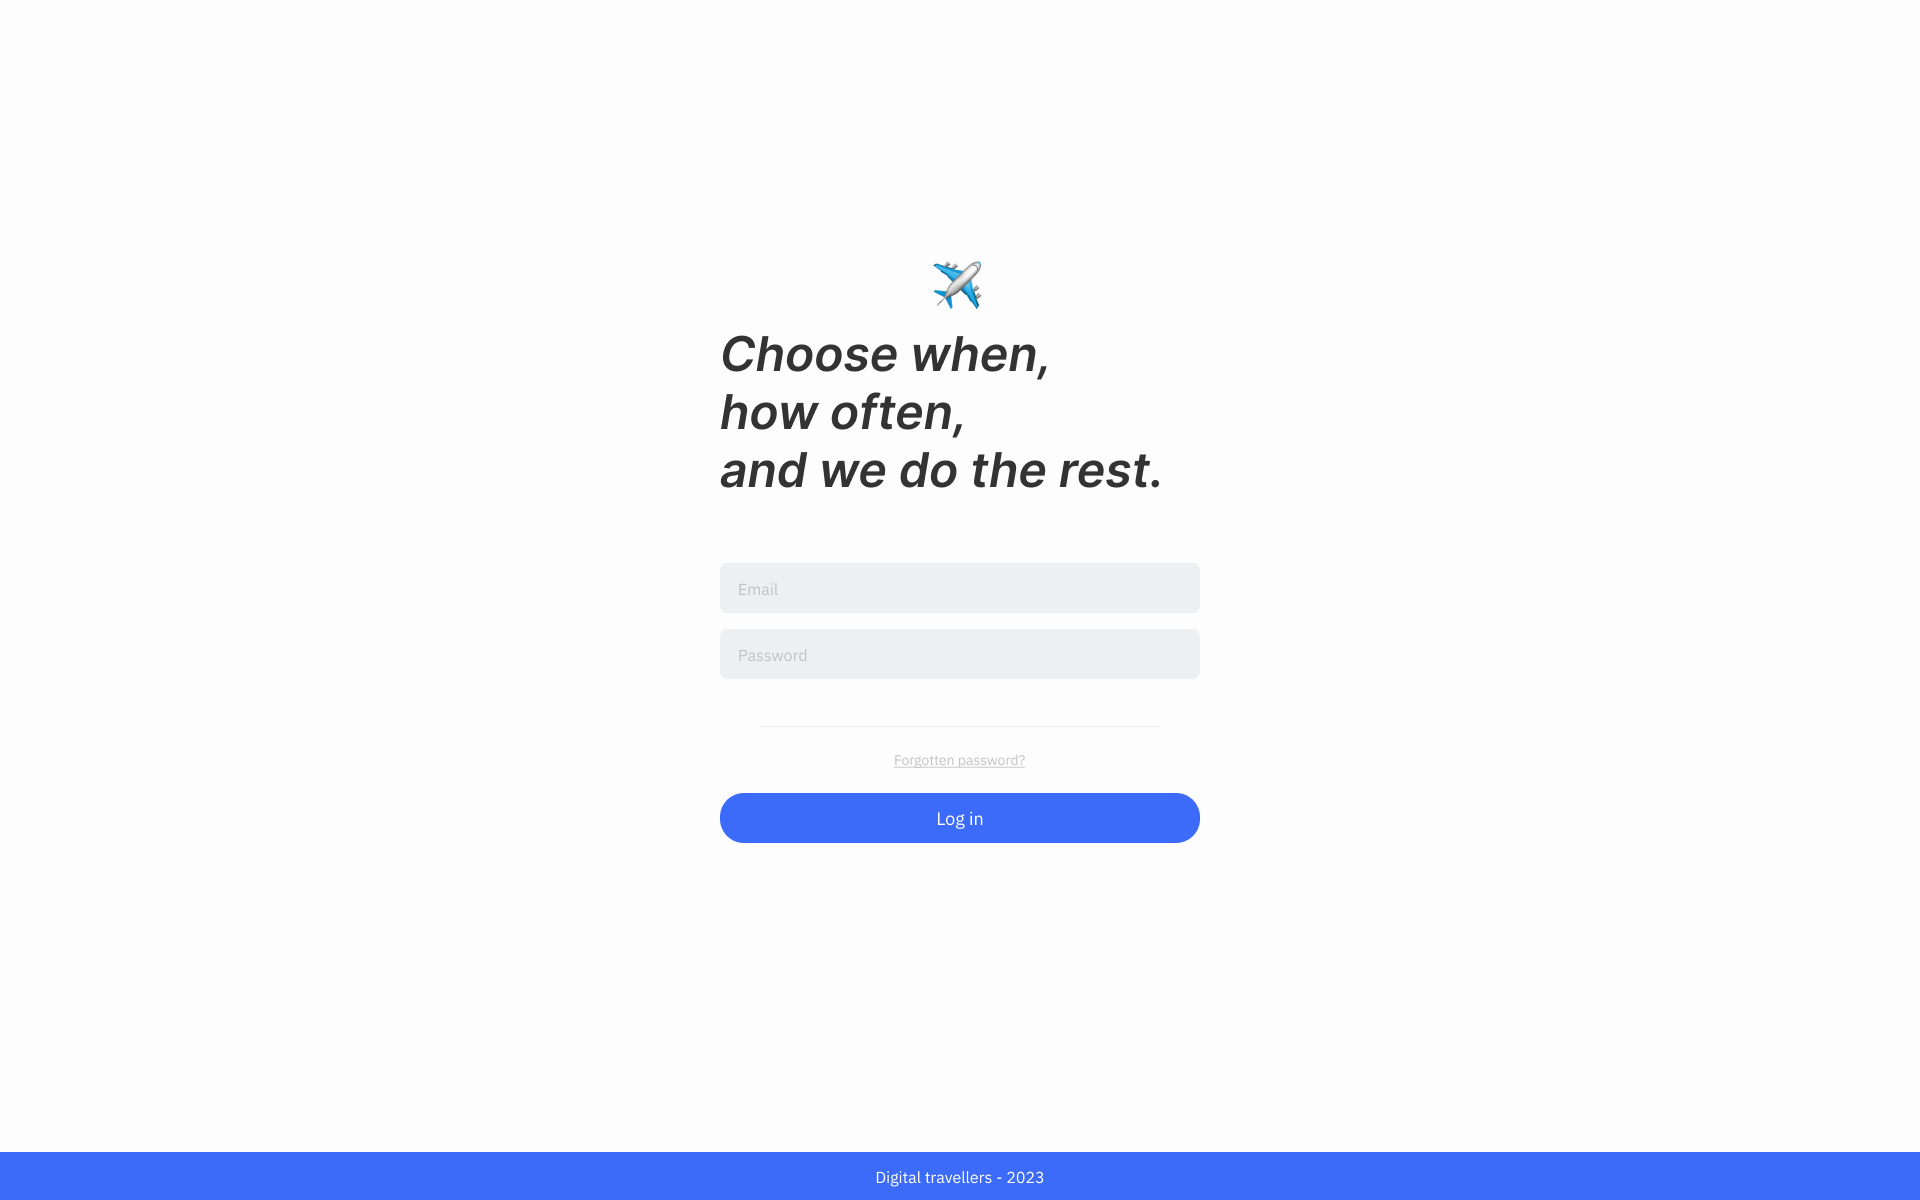
\includegraphics[width=\textwidth]{./assets/designs/login-desktop.png}
	\caption{Login page design}
\end{figure}
\begin{figure}[H]
	\centering
	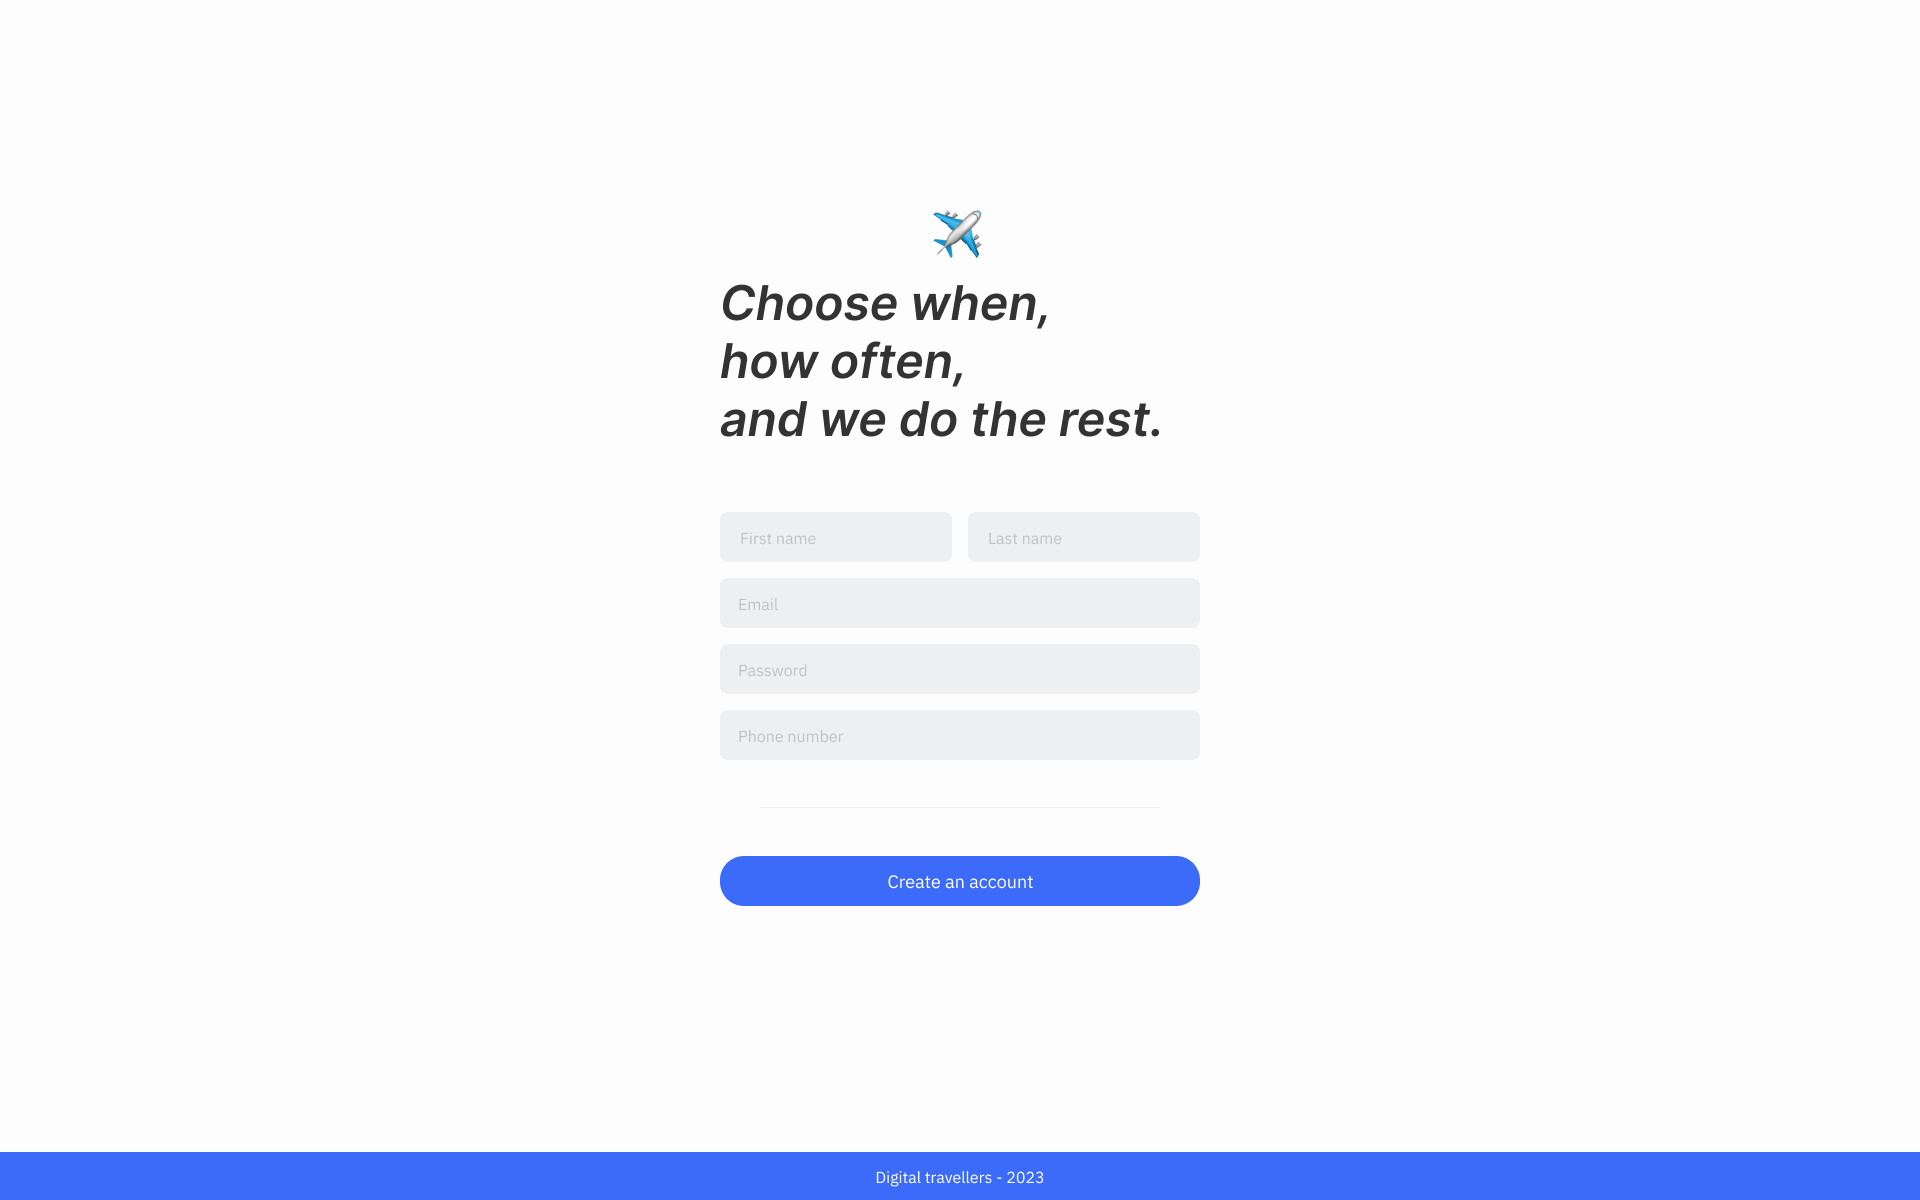
\includegraphics[width=\textwidth]{./assets/designs/signup-desktop.png}
	\caption{Sign-up page design}
\end{figure}
\newpage
\subsection{Authenticated pages}
Once the user has been authenticated, it will be redirected to the dashboard
page. The dashboard page is the page from which the user is going to be able to
see the list of travels created. As explained, the designs do not reflect the
correct model, as the travel's model was updated during the development of the
application.
\\
It should also allow the user to interact with the created alerts, being able to
modify them or remove them, as well as being able to create new ones.
\begin{figure}[H]
	\centering
	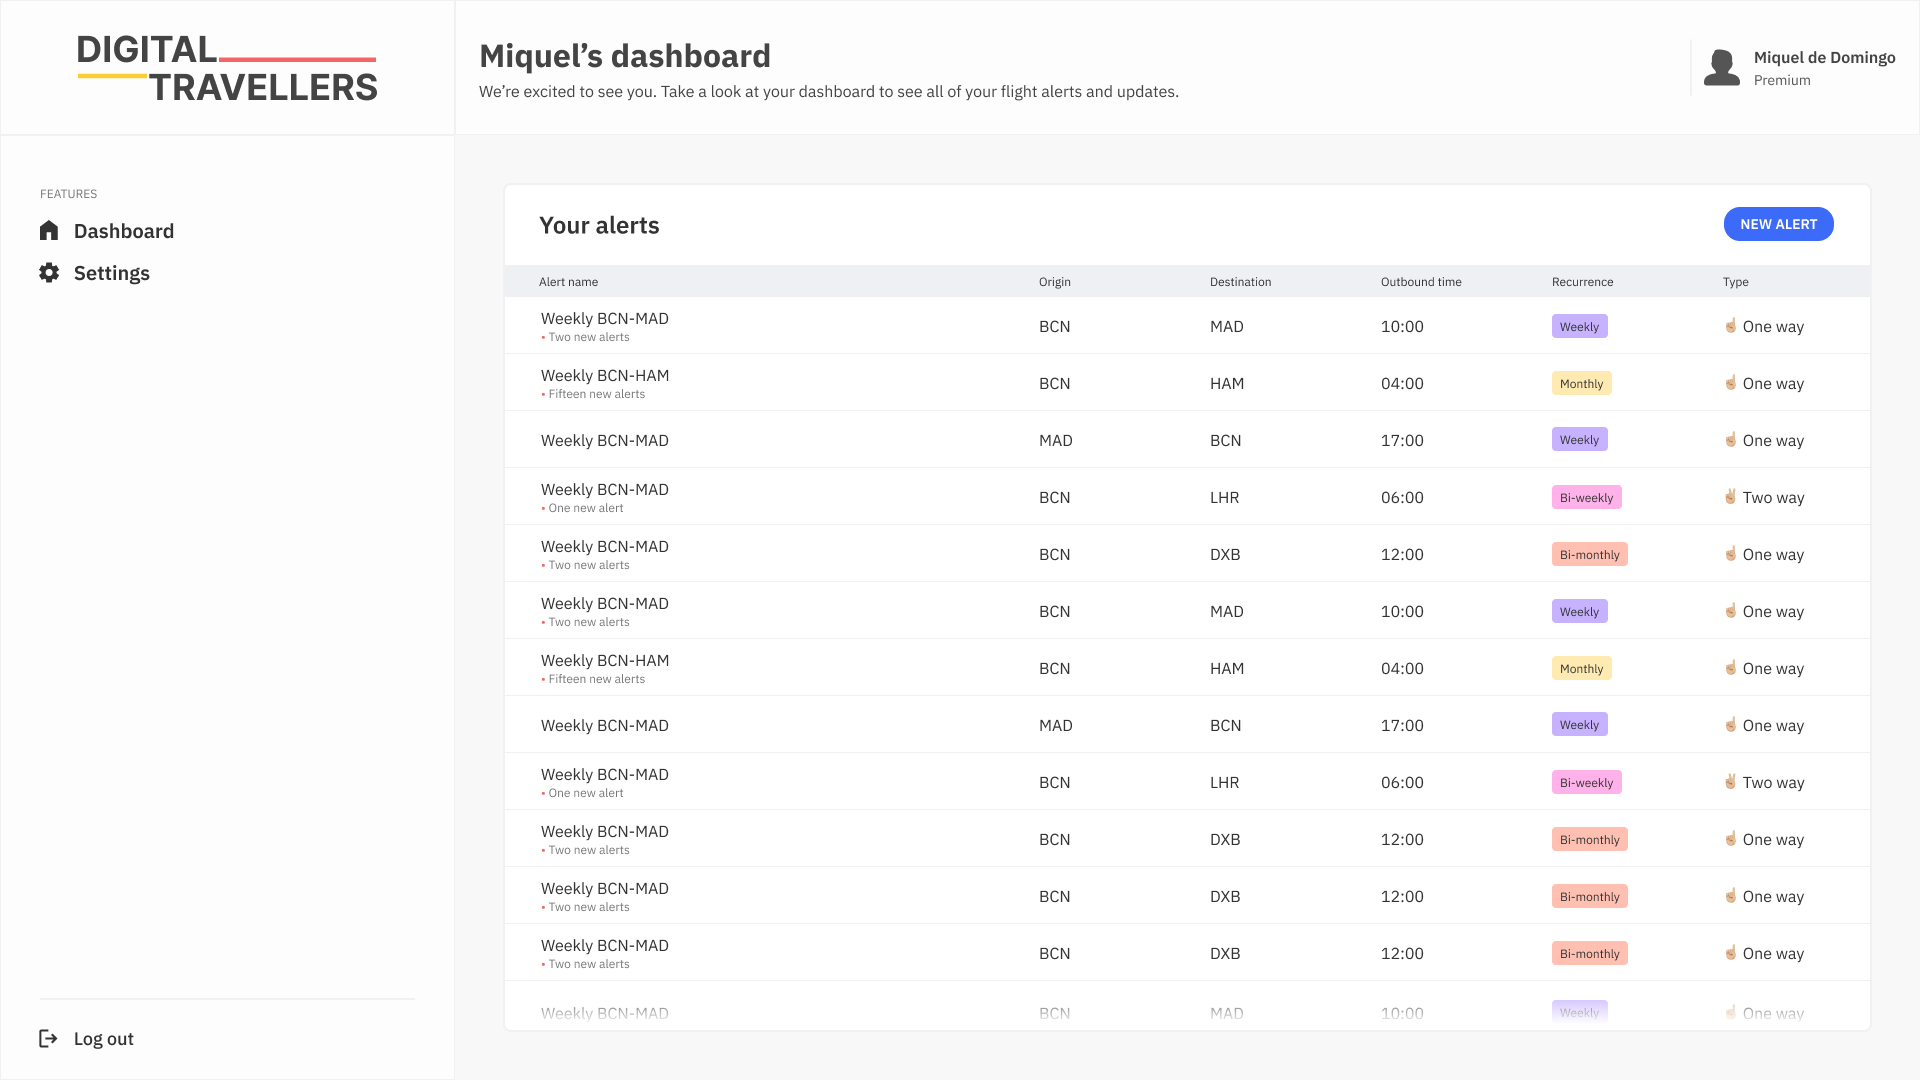
\includegraphics[width=\textwidth]{./assets/designs/dashboard-desktop.png}
	\caption{Dashboard page design}
\end{figure}
\newpage
The other authenticated page, which would only be developed if there was enough
time, is the settings page. This page allows the user to update their
information.
\begin{figure}[H]
	\centering
	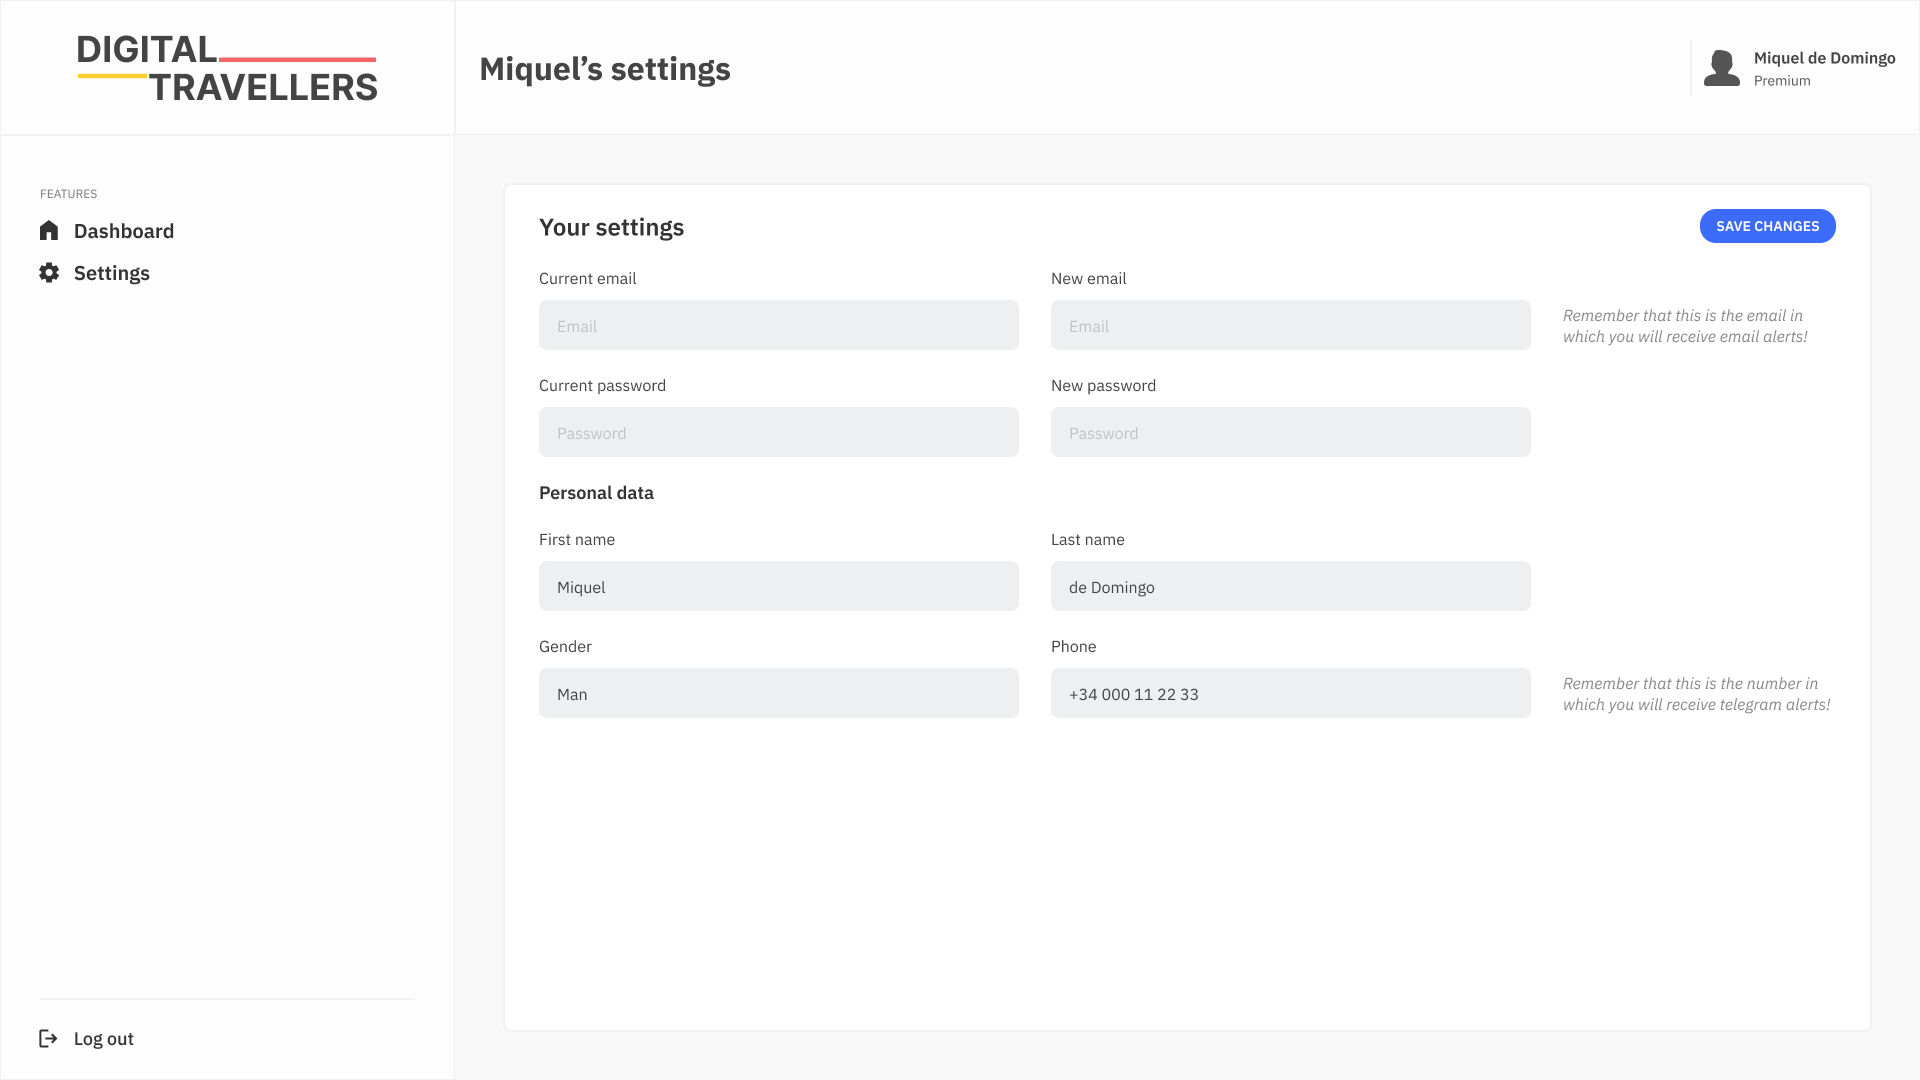
\includegraphics[width=\textwidth]{./assets/designs/settings-desktop.png}
	\caption{Settings page design}
\end{figure}
\newpage
\subsection{Mobile first}
Last but not least, the mobile designs were a crucial aspect of the overall
design strategy. The objective was to simplify the mobile design to minimize
absolute differences between the desktop and mobile versions. The rationale
behind this approach was to reduce complexity in the development process. As
fronted developers, we often encounter intricate designs that result in a
complex, challenging and hard to maintain codebase. With the MVP approach in
mind, the focus was creating a design that promotes component and layout
reusability in the frontend.
\\[8pt]
By aligning the mobile designs with the overall design principles, the goal was
to achieve consistency and coherence across the different screen sizes and
devices.
\begin{figure}[H]
	\centering
	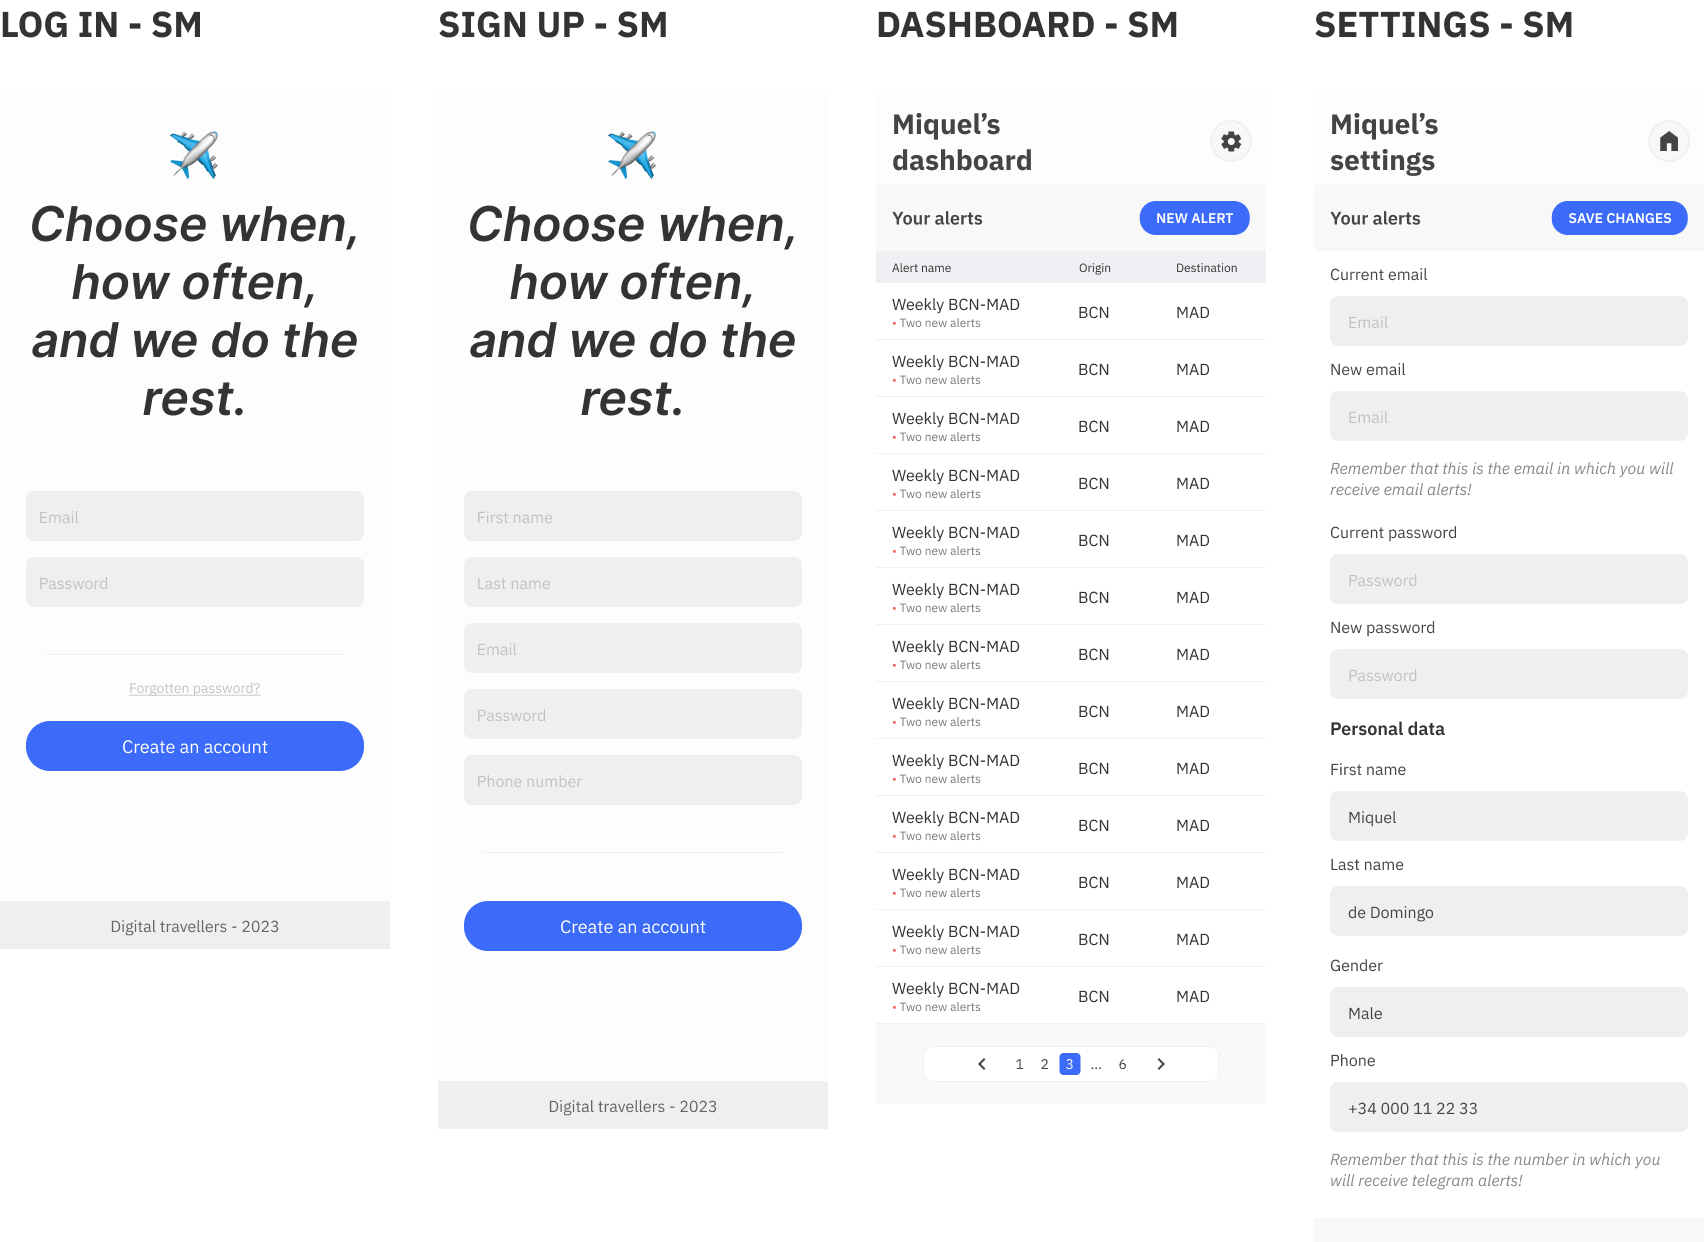
\includegraphics[width=\textwidth]{./assets/designs/design-sm.png}
	\caption{Mobile designs for the 4 initial pages of the application}
\end{figure}
\section{Domain development}
With the designs in mind, the frontend was ready to start being developed. In
the development process, it has been observed that a significant portion of new
tickets or tasks revolve around adding new features or making updates within the
domain package, as a starting point. This package serves as the heart of the
application, encapsulating the core business logic. As a result, the first phase
of addressing a ticket often involves making changes within the domain package.
\\[8pt]
As it has been repeated throughout the project, the goal is to ensure a robust
and maintainable codebase. Therefore, the development of the domain package
strictly adhered to the principles of the hexagonal architecture. Accordingly,
the development has followed a sequential order, beginning with the domain
layer, followed by the application layer, and concluding with the infrastructure
layer.
\\
Moreover, initial tasks required more time and decision-making, as the
codebase had nothing written yet.
\\[8pt]
To ensure the reliability and functionality of each layer, comprehensive testing
has been added. Tests have been developed per layer, allowing for thorough
validation of the domain, application, and infrastructure components. Within the
domain layer, particular emphasis has been placed on testing entities with
complex business logic, as these entities play a central role in driving the
application's functionality. Simpler entities or those closely intertwined with
other layers are covered by more comprehensive and complex tests, ensuring their
validation within a broader context.
\\
It is also important to distinguish between the tests developed for each layer:
\begin{enumerate}[label = -]
	\item\textbf{Unit testing}. Unit testing allows the developers to test a
	single unit of code, excluding all the other that depends on or are
	attached to it. Therefore, the domain and application layer have been
	tested with unit tests.
	\item\textbf{Integration testing}. Integration testing allows the developers
	to test broader units of code, in this case, integration testing has been
	used for each querier in the domain layer. Therefore, the tests ensure the
	behaviour of the code, as a whole.
\end{enumerate}
End to end or acceptance test have not been developed because the domain package
does not require of such testing. Since it is not attached to any framework,
database nor similar, there is little benefit in having such tests. Furthermore,
the configuration of such tests tends to be really tedious, complex, and time
demanding.
\\[8pt]
To sum up, the development of the domain package has generally been really
straightforward, and it has only required the communication between the frontend
and the backends to know the expected models to received and to be sent.
\section{Implementing the frontend}
The designs also helped define the small unit of components, that, instead of
being in the application package, should be in the UI package. As explained
before, the UI package is responsible for having the implementation of the
components for each frontend framework it is used within the frontends.
\\[8pt]
Before diving into the task at hand, the first step was to analyse the design
and identify which components needed to be added to the UI React package. It was
also checked if there was any existing component that could be repurposed to
meet the requirements. However, there were cases where the existing components
did not fully meet the needs of the task. In such situations, it was necessary
to determine whether the desired functionality was something generic, applicable
to future tasks, or if it was specific to the current task.
\\
For generic features that we anticipated would be needed in future tasks, they
were added to the UI package. This allowed the team to reuse the shared logic
and streamline future development. On the other hand, if the feature was specific
to the current task, the composition over inheritance principle was followed.
This means that necessary features where added to the shared component using
composition, without relying on complex inheritance structures. It is also
important to not that, if the feature required any type of domain dependency, it
could not be added to the UI package, as such has to be domain independent. It
indirectly also adds a requirement for all the components that are developed in
the UI package, which is that they should be extendable by nature.
\subsection{Identifying components}
The goal of this section is to explain how the process of identifying components
has been done. This explanation will be covered for the one of the
authentication pages and the dashboard page. As explained previously, this is
the first step in order to define whether a component should be developed and
maintained inside the application, or be part of the shared UI package. In this
case, most of the components exposed in this section are part of the UI package.
\\[8pt]
When developing a component for a library in React, there are several
considerations that the developer has to keep in mind. All the components should
be designed to be domain-independent, as it is also one of the requirements
exposed in previous chapters. This promotes the reusability of the components
and ensures that the component can play different roles across different
projects.
\\
Furthermore, it is crucial to make the component extendable and composable. By
designing the component with a modular or atomic\footnote{Atomic design is a
	term commonly used in React and component based frameworks. The goal is to
	design the components in the smaller atoms as possible.} approach, it becomes
easier to add new functionalities and customizes its behaviour as per specific
requirements. This allows developers to build upon the component's foundation
without the need to modify its core implementation, leading to more flexibility,
adaptability, and speed of development.
\\
Maintainability is another key aspect to consider. The component must be
structured in a way that is easy to understand and maintain over time. Clear and
concise code, along with proper documentation and consistent naming conventions
can greatly contribute to the long-term maintainability of the component.
\\
Additionally, the component should be designed with testing in mind. It should
be easy to write unit tests for the component's functionality, ensuring that it
performs as expected and minimizing the risk of introducing bugs during
development or future updates. By incorporating testability into the component's
design, it becomes easier to validate its behaviour and provide a more robust
user experience.
\\[8pt]
In the following sections, we will discuss the implementation of integration
testing versus unit testing for components. I have not been particularly
inclined towards implementing unit testing for components in the past, mainly
because it can be relatively complex due to the numerous dependencies that
components often have (such as state and the need for other components).
However, when it comes to developing a library, it becomes crucial to test each
component individually since they should represent standalone units. Therefore,
it makes sense to incorporate unit testing specifically for components, while
integration testing may not be as necessary in this context.
\subsubsection{Sign-up page}
The sign-up design is really basic and intuitive. The idea is to have a centred
form that requests all the necessary user information to create the account. The
following image shows the different components identified, as well as the
automatic centring of the form.
\begin{figure}[H]
	\centering
	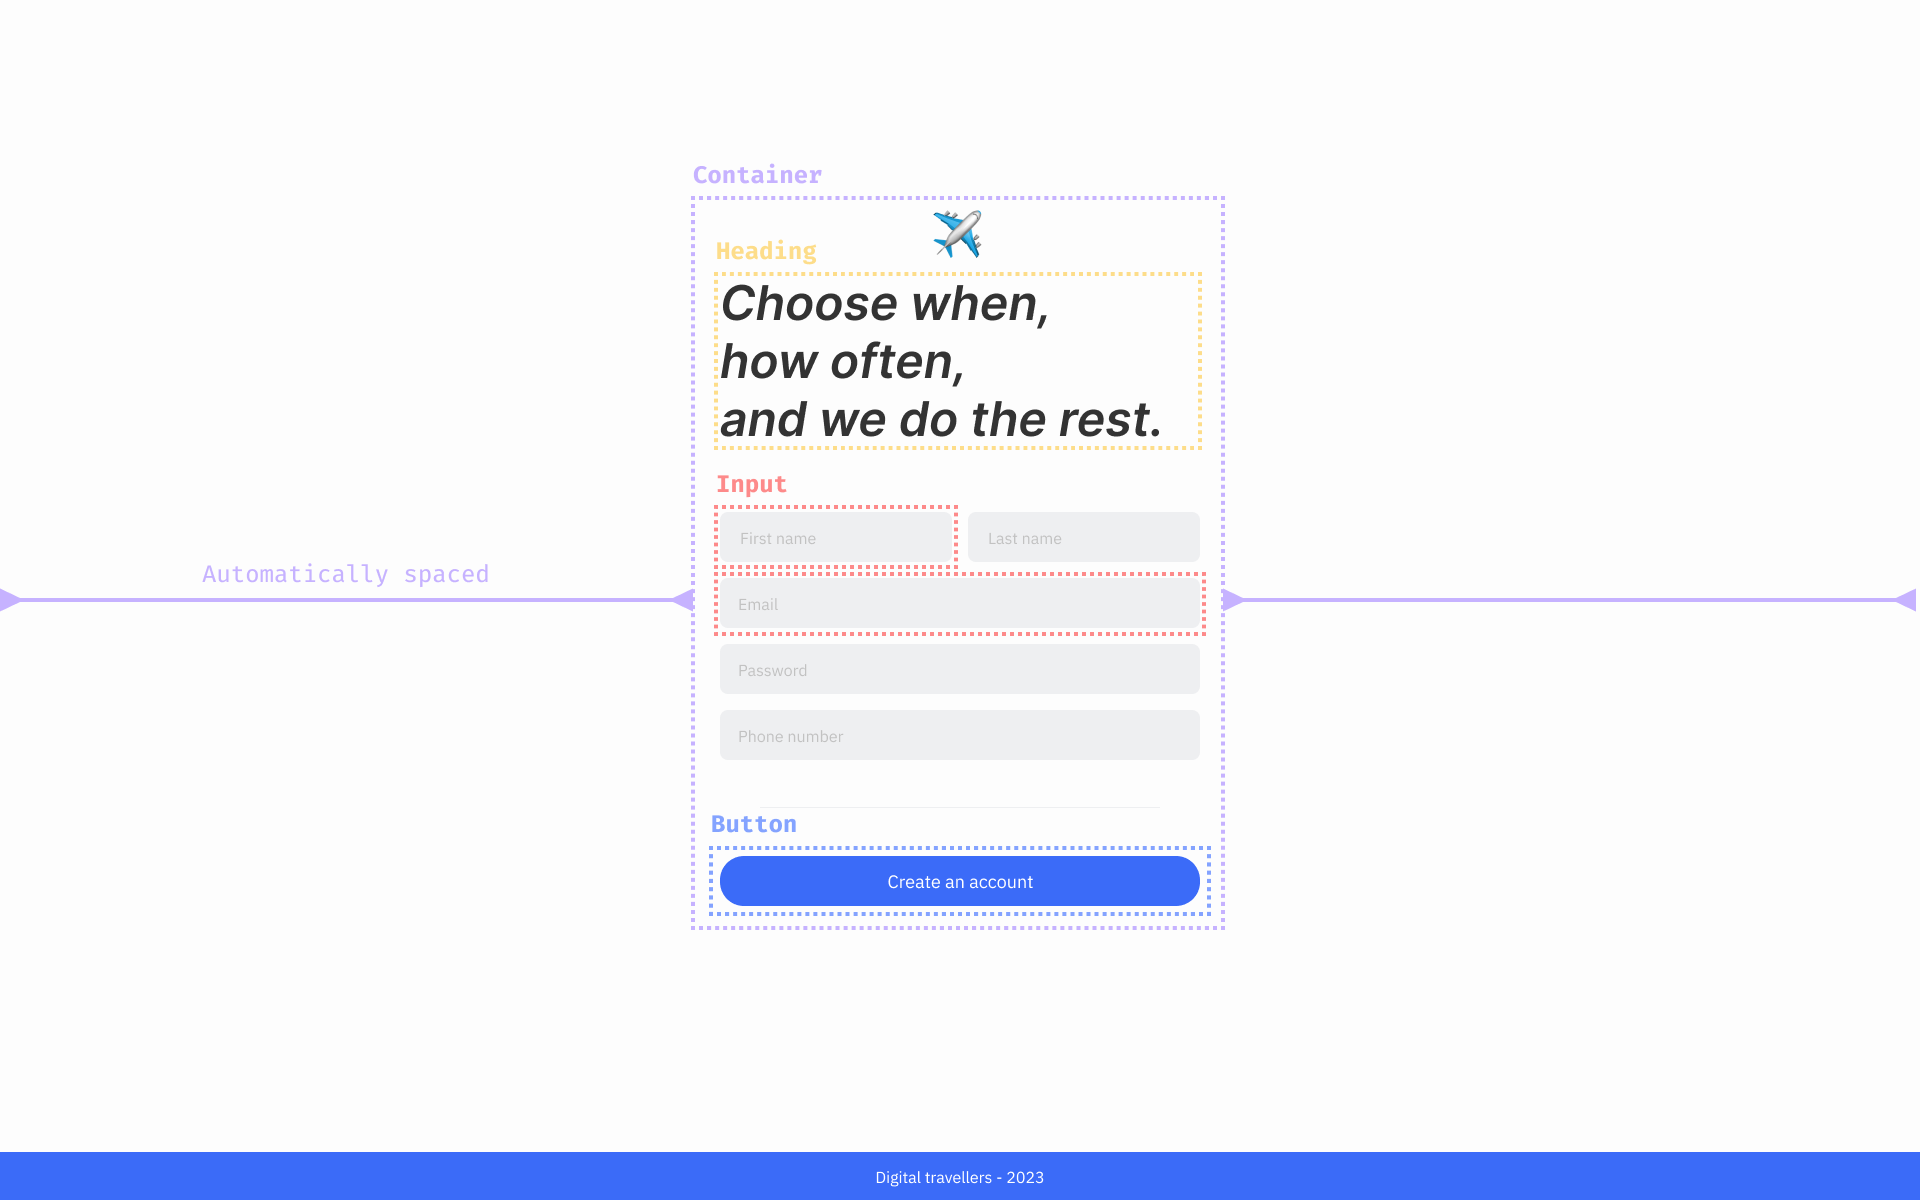
\includegraphics[width=\textwidth]{./assets/designs/sign-up-components.png}
	\caption{Component destructuring of the sign-up page}
\end{figure}
First aspect that can be seen is the container that wraps the form, ensuring
its maximum width and allowing the form to be centred. The same container will
be used for the login page. The container is a common component that it is used
to wrap content and limit its width. In this case, the container has been
defined in order to have different sizes, being able to be set depending on the
needs. For instance, the same container can be used in a third page, yet instead
of having this \emph{condensed} size, the developers may need to expand it to
fit a larger screen. Last but not least, it is the container's responsibility to
be automatically centred, independent of its size and the size of its parent.
\\[8pt]
Inside the container, it is first seen the heading of the form. Modern
applications tend to use a great variety of font sizes, each being a different
heading, text, subtitles or even captions. HTML contains six types of headers,
from \texttt{h1} to \texttt{h6}. Headers play an important role when talking
about semantic HTML. It is important to use proper headers for reasons such as
improved SEO or better accessibility (helping screen readers and other
accessibility tools). Planning in advance, when developing the typography, I
decided to design the entire typography system. The following typography styles
have been implemented:
\begin{figure}[H]
	\centering
	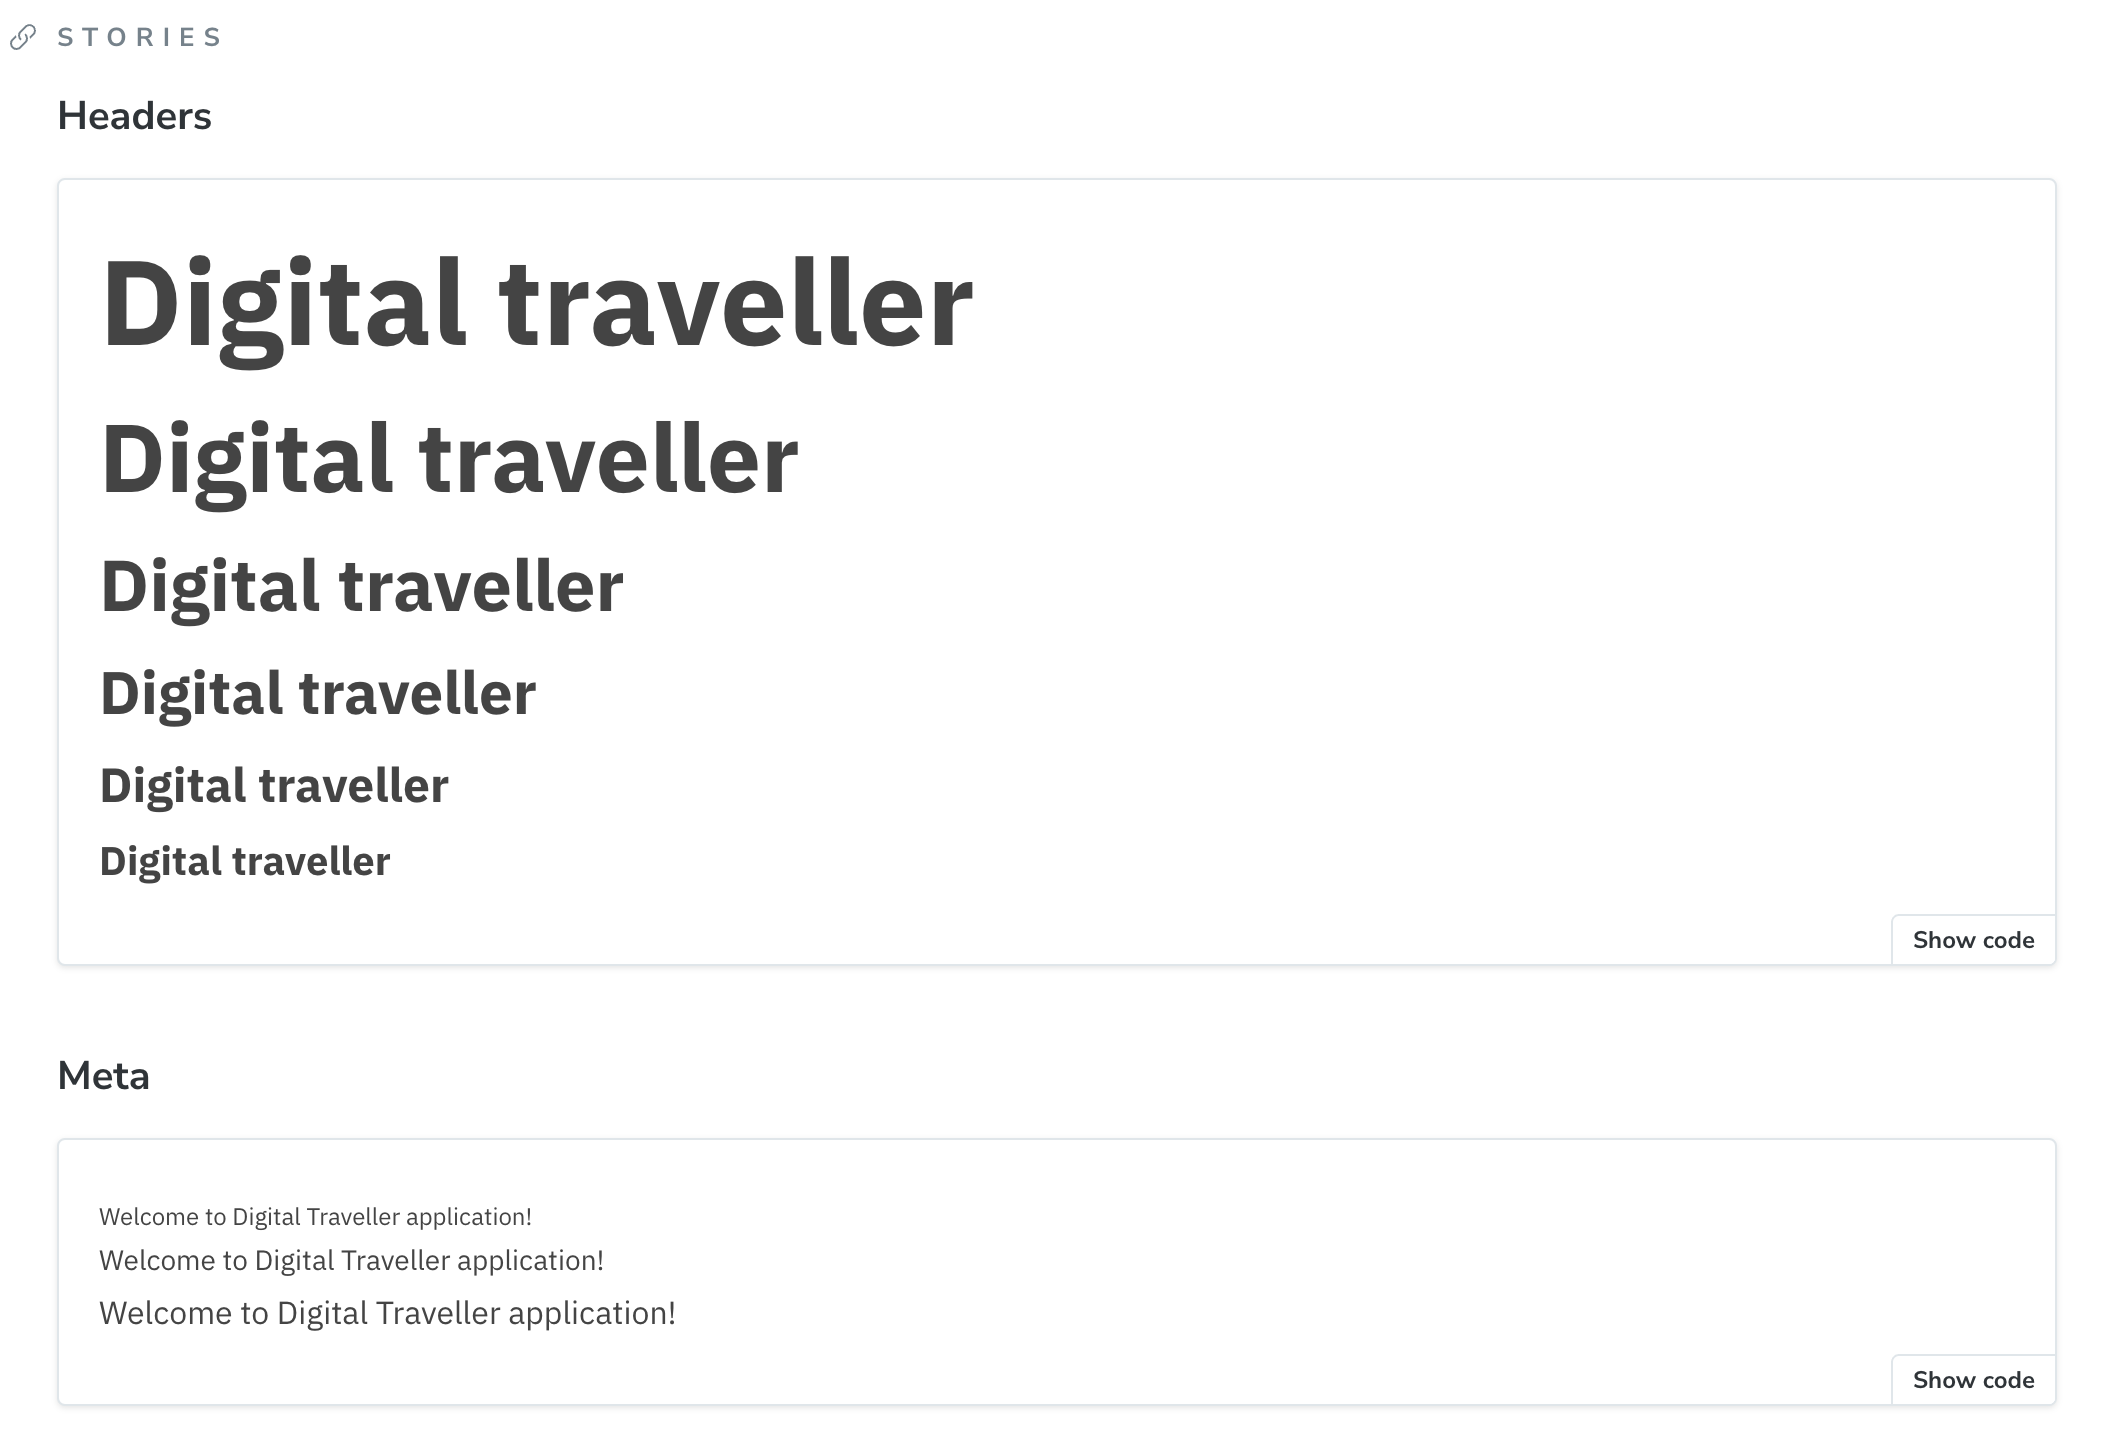
\includegraphics[width=\textwidth]{./assets/designs/typography.png}
	\caption{System design's typography}
\end{figure}
The implementation consists of 6 components, one for each HTML heading variant,
and 1 component with 3 variants (extra-small, small and medium, which is the
default text). The reason why the headings are 6 components instead of one with
six variants is because each component internally renders from \texttt{h1} to
\texttt{h6}. Needless to say, these components are extendable and customizable,
meaning that they can be adapted to the needs of the design.
\\[8pt]
Another noteworthy aspect to mention is the library used for visualizing and
testing the components, which is Storybook. Storybook provides a dedicated
environment for showcasing components in isolation, allowing developers to
interact with them and visualize their various states and variations. It serves
as an invaluable tool for component development, as it enables rapid
prototyping, visual inspection, and iterative design improvements.
\\
With Storybook, developers can create a comprehensive library of reusable
components, each with its own story or scenario. These stories represent
different use cases or variations of the component, showcasing its behaviour and
appearance in different contexts. This approach not only helps in the visual
testing of components but also serves as documentation, providing examples and
usage guidelines for other developers.
\\
Furthermore, Storybook allows for easy interaction with components through its
add-on ecosystem. Add-ons provide additional functionality and features, such as
knobs for dynamically tweaking component props, actions for capturing user
interactions, and accessibility testing to ensure components are usable for all
users.
\\
By leveraging the power of Storybook, developers can streamline the component
development process, improve collaboration, and ensure the visual integrity and
quality of their components. It aids in building components that are visually
appealing, easy to understand, and thoroughly tested, ultimately contributing to
the overall success of the library. Additionally, it serves as documentation for
the package.
\\[8pt]
In this case, the image is displaying the story of the typography, which
involves the two components that are part of the typography.
\\[8pt]
Next component is the input component, which provides an excellent demonstration
of the concepts of composition and extensibility in component development. It
also plays a crucial role in user interaction and data input, making it
essential to consider various aspects such as accessibility, reusability,
extendability and performance\footnote{In React, it is very important to pay
	attention to the performance of inputs and forms, as bad practises or incorrect
	patterns may lead to an excess of renders, which will reduce the performance of
	the application.}.
\\
When it comes to accessibility, the input component must adhere to best
practices to ensure that it can be used by individuals with disabilities. Even
though it may seem out of scope from the MVP, considering accessibility in
advance may simplify future work. By prioritizing accessibility, the input
component becomes inclusive and usable for a wider range of users, from the
beginning.
\\
Extensibility is a crucial aspect for the input, in order to accommodate
potential future changes or new requirements. By following a modular design and
implementing clear separation of concerns, it becomes easier to extend the
functionality without disrupting its existing behaviour. An example would be the
addition of features like auto-suggestions, masks, or integrations with external
libraries. Such features should be added with minimal impact on the existing
code base.
\\
For example, a library will be used in order to ensure the maximum performance
of forms, which is named \texttt{react-hook-form}. The input component should be
able to adapt to this library by default, as it should with any other.
Furthermore, it should not be attached to any library. The fact of having such
simple components, ensures that its basic behaviour can easily be tested,
reducing test complexity and improving readability.
\\[8pt]
Finally, the button component. As with the input component, the button should be
as extendable as possible, while being accessible for all users.
\subsubsection{Dashboard page}
The dashboard page contains more complexity and logic than both of the
authentication pages. Nonetheless, in this section only the main content will be
focused, as the layout of the page will be explained in the next section.
\begin{figure}[H]
	\centering
	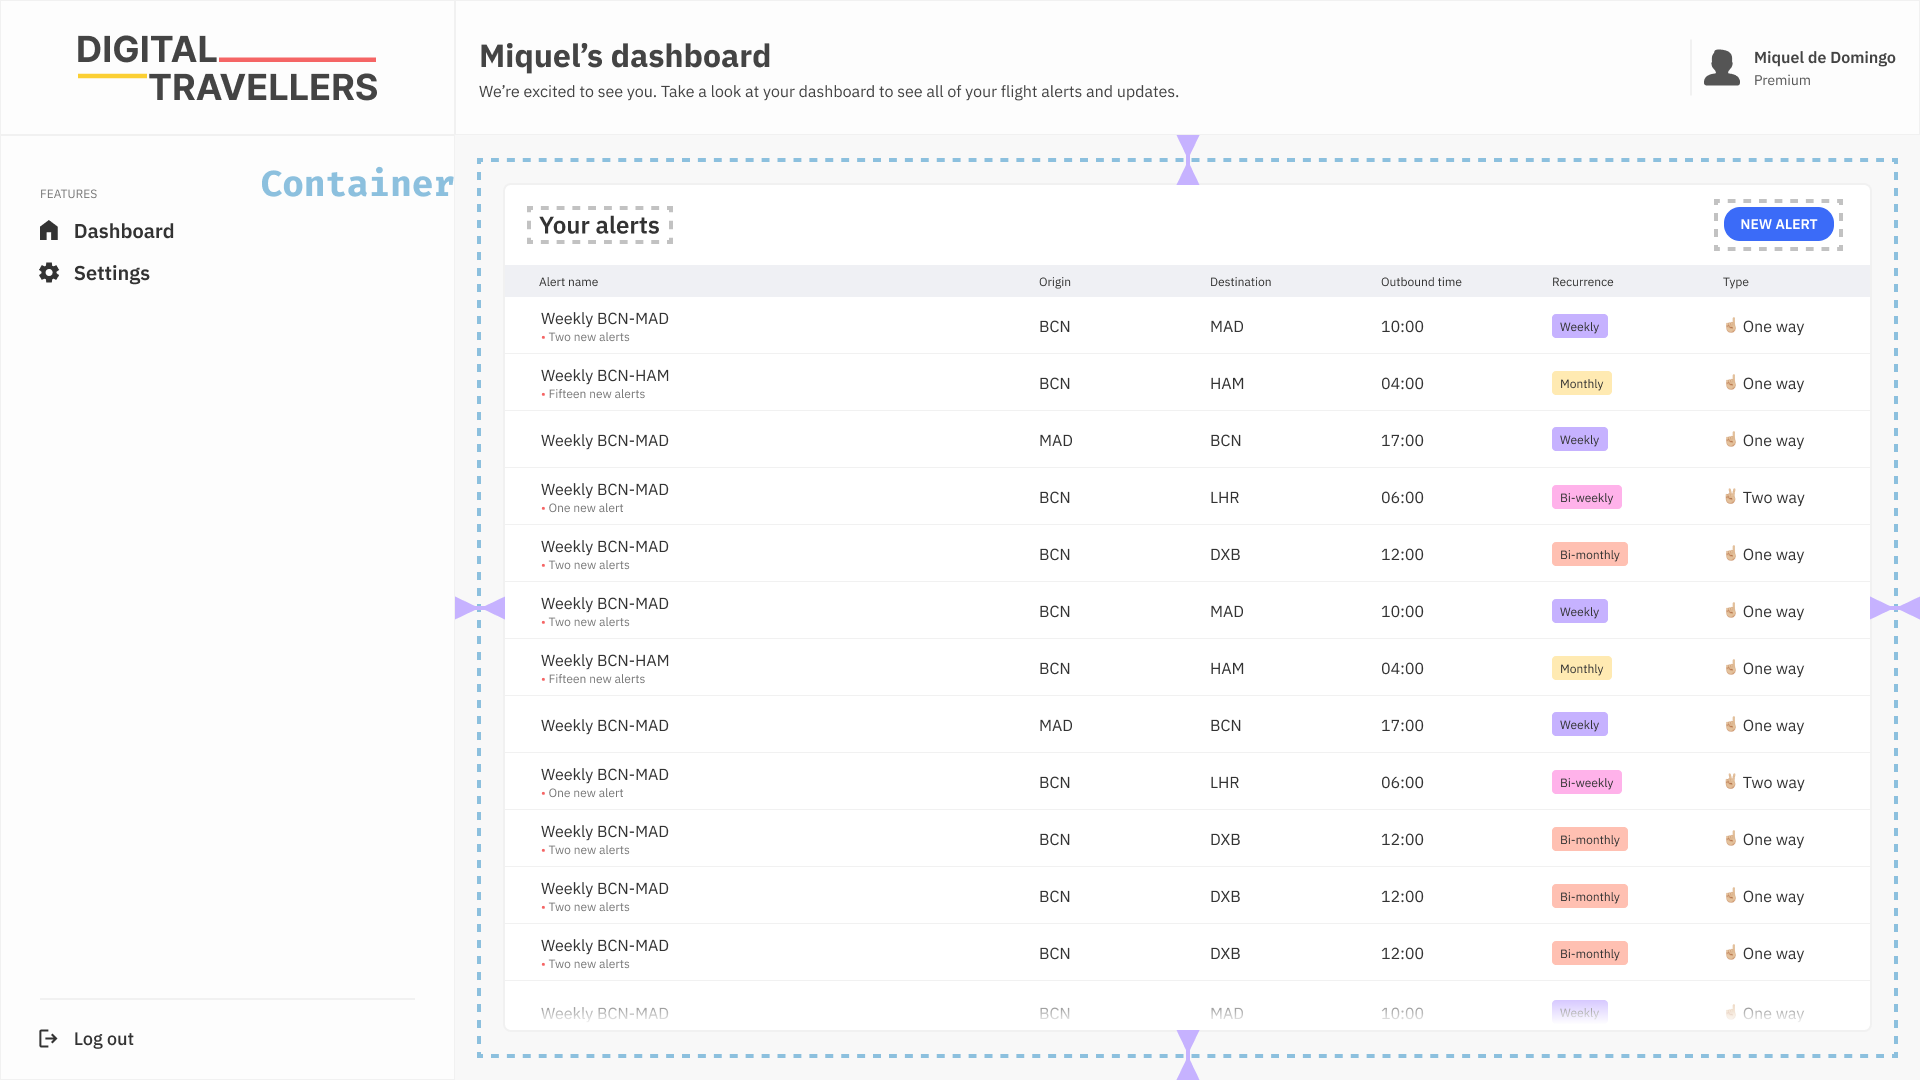
\includegraphics[width=\textwidth]{./assets/designs/dashboard-web-container.png}
	\caption{Component destructuring of the dashboard content}
\end{figure}
The content of the page consists of a card that will be centred and
proportionally spaced from top, bottom, left and right. This card usage is very
common in order to catch the attention of the user to the middle of the
dashboard, where the alert list or table is contained.
\begin{figure}[H]
	\centering
	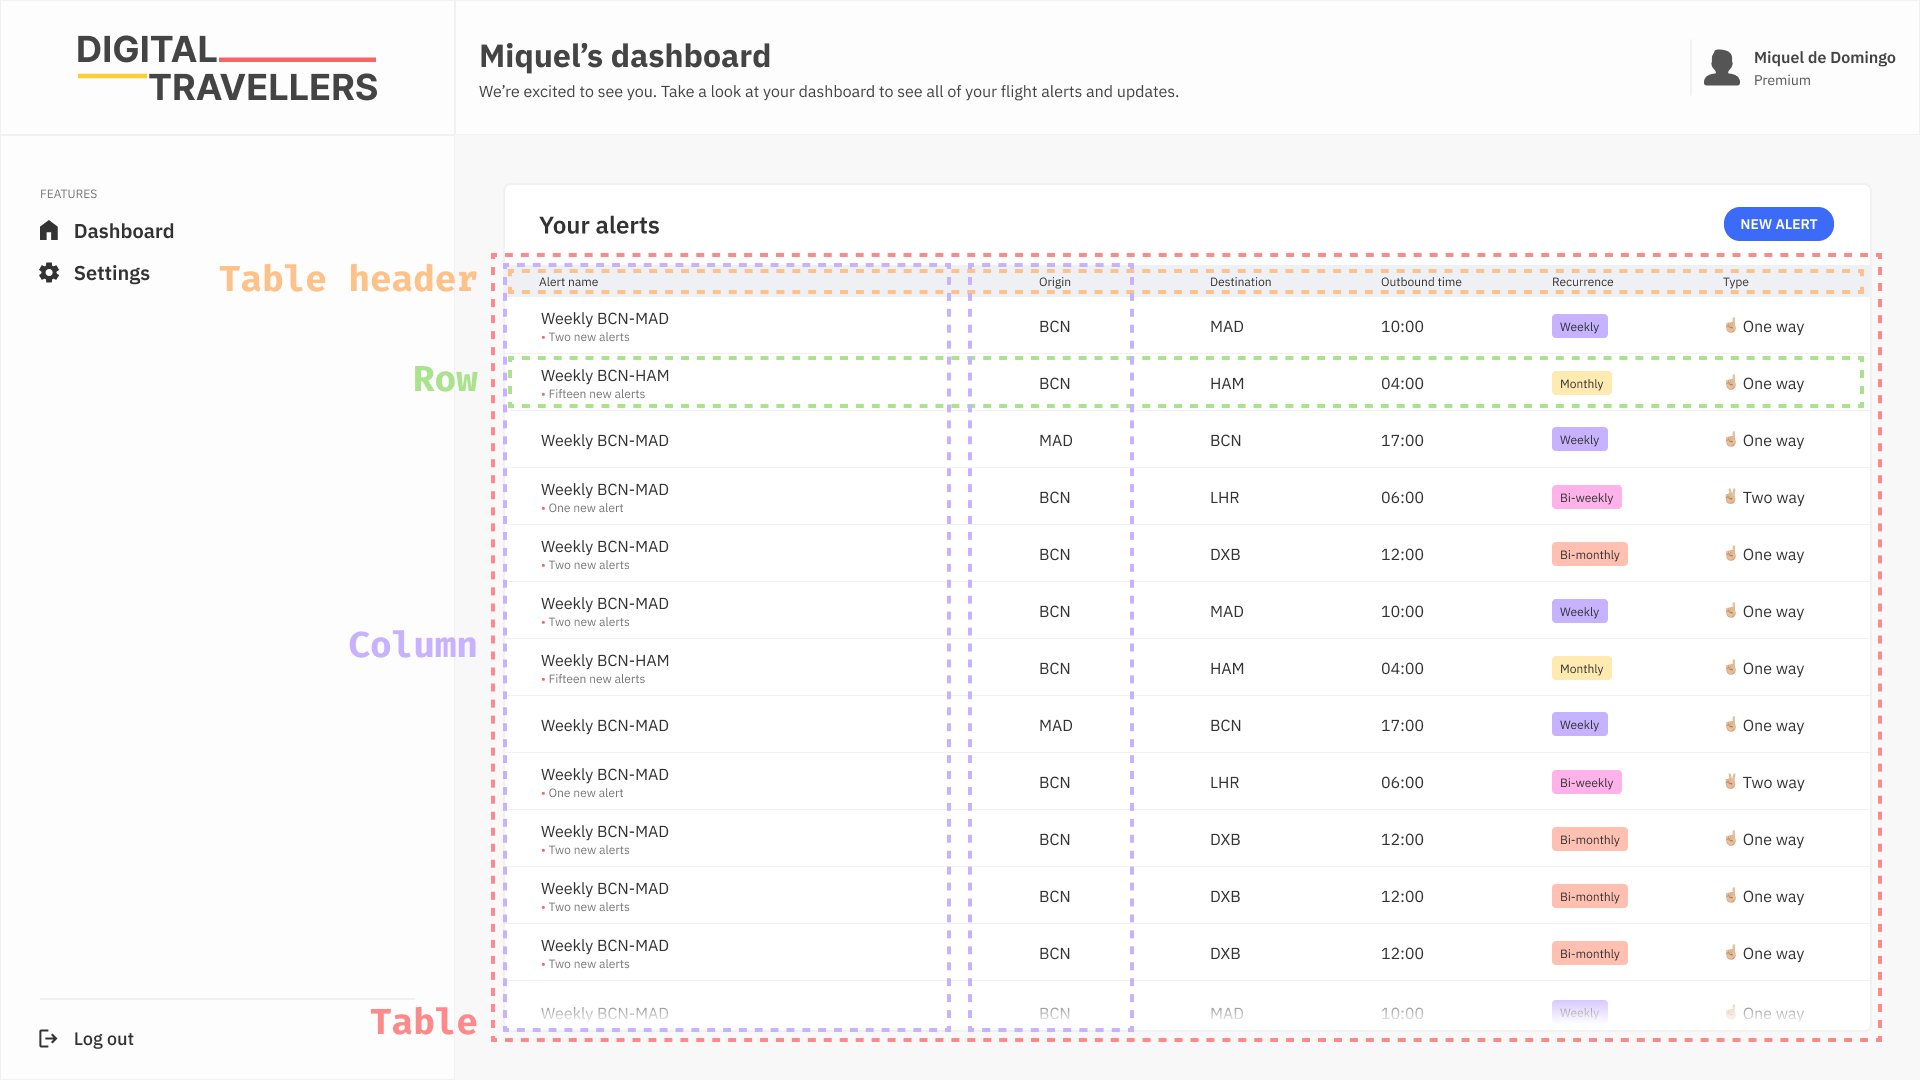
\includegraphics[width=\textwidth]{./assets/designs/dashboard-web-table.png}
	\caption{Component destructuring of the dashboard table}
\end{figure}
The table is a more complex component, as it should be responsive and ensure all
accessibility requirements, and for this case, I opted to divide the table in
the following components\footnote{This table has been inspired in the
	implementation of \href{https://mui.com/material-ui/react-table/}{\texttt{mui}'s
		library.}}, some of them being marked in the design, and some not:
\begin{enumerate}[label = -]
	\item\textbf{Table container} (not marked in the image). The table container
	it is a container that it is used to provide a certain styling to the
	table in order, for example, to allow the table header to stick when
	scrolling down.
	\item\textbf{Table} (marked in the image). Represents the actual table,
	rendering a \texttt{table} element to the DOM.
	\item\textbf{Table head} (marked in the image). Represents the table header,
	which has a different style than the table body rows. It renders a
	\texttt{thead} element.
	\item\textbf{Table body} (not marked in the image). Represents the table
	body, where the content should be rendered. It renders a \texttt{tbody}
	element.
	\item\textbf{Table row} (marked in the image). Represents a row of the table
	and should be used both for the header and the body. It renders a
	\texttt{tr} element as well as providing the alternate style of one row
	darker than the other.
	\item\textbf{Table cell} (not marked in the image). Finally, the table cell
	that is the component of the content to display for each position of the
	table. It renders a \texttt{td} element.
\end{enumerate}
The goal of having these many components is for the end developer to be able to
construct the table based on its needs. Each component can be extended and
customized, and some of them are not even required for the table to work, yet
they provide certain utilities that may be necessary. For example, a design may
not require of a table header component and such should not represent any
inconvenience when not incorporated.
\\
Accessibility should be a top priority. Tables should be designed in a way that
allows users of assistive technologies, such as screen readers, to navigate and
understand the table structure and content. This includes providing proper table
headers, using semantic markup, and ensuring that data cells are associated with
their corresponding headers. Additionally, tables should be designed to be
responsive, allowing users to interact with them effectively on different
devices and screen sizes.
\\
Data representation is another important consideration when working with tables.
The table component should provide options for sorting, filtering, and
pagination to handle large datasets effectively. These features enhance the
usability of the table, allowing users to find and interact with the data more
efficiently. Additionally, it is important to consider accessibility features
such as keyboard navigation and providing alternative text for table visuals,
such as data charts or graphs. However, due to the complexity of some of these
features, they have not been included as part of the MVP.
\begin{figure}[H]
	\centering
	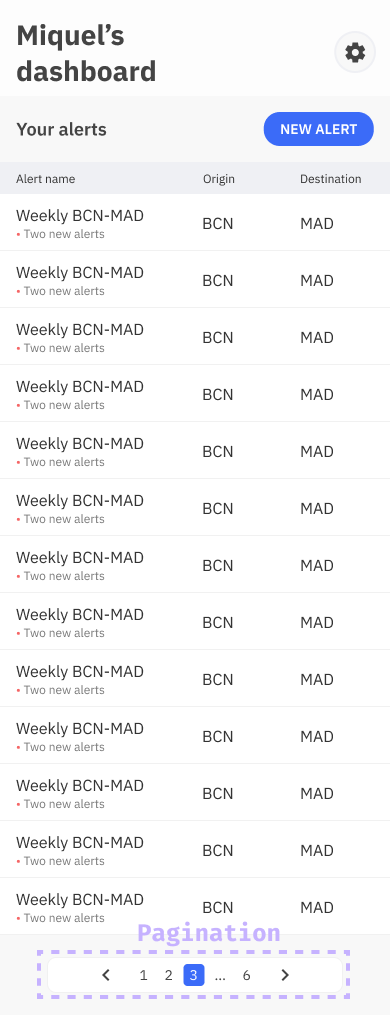
\includegraphics[width=0.25\textwidth]{./assets/designs/dashboard-sm-pagination.png}
	\caption{Component destructuring of the dashboard content}
\end{figure}
Finally, the mobile version was initially designed with a pagination component.
This component has not been developed as I believe it does not provide the best
user experience for mobile users. If the pagination existed, the user would have
to scroll to the bottom and then change the page. However, if instead of
pagination, infinite scroll is used, it provides a better user experience.
Nonetheless, the final implementation has been done by loading all the travels.
Implementing infinite scroll or pagination, could be done in a second version,
after the MVP.
\subsection{Layouts for performance}
Next.js focuses mostly in server-side rendering and static site generation. One
of the challenges developers often face when working with Next.js is creating
persistent layouts that do not re-render the entire UI when navigating between
pages. This is because, by default, Next.js re-renders the entire UI every time
a link is clicked, which can lead to a less-than-optimal user experience.
\\
This section will focus on the analysis of the layouts for the designs, so that
they can be reduced throughout the application.
\\[8pt]
In Next.js, layouts \cite{nextjs-layouts} refer to a concept where you can define
a common structure or template for your pages. A layout acts as a wrapper
component that encapsulates the content of multiple pages, providing consistent
styles, navigation, headers, footers, or any other shared elements. It allows
you to define a higher-level structure that can be applied to multiple pages in
your application.
\\
Layouts are important because they bring several benefits to the development
process and user and developer experience:
\begin{enumerate}[label = -]
	\item\textbf{Consistency}: By using layouts, you can ensure a consistent UI
	across multiple pages. This is especially useful for elements like
	headers, footers, or sidebars that should remain the same throughout the
	application. Users will have a unified experience as they navigate through
	different pages, having this shared components not disappearing and
	appearing on a page change.
	\item\textbf{Code reusability}: Layouts promote code reusability by
	providing a central place to define them. Instead of repeating the same
	code in every page, you can encapsulate it within a layout and reuse it
	across multiple pages. This saves development time and reduces code
	duplication, as well as improving maintenance and simplifying testing.
	\item\textbf{Easier maintenance}: When you have a common layout for multiple
	pages, making changes or updates becomes easier. The developer only needs
	to modify the layout component, and the changes will be automatically
	reflected in all pages that use that layout. This makes maintenance more
	efficient and reduces the risk of introducing inconsistencies or errors.
	\item\textbf{Flexibility and customization}: Layouts allow for flexibility
	and customization. You can have different layouts for different sections
	or types of pages in your application. For example, you might have a
	different layout for the homepage, an authenticated user dashboard, or a
	landing page. This gives you the freedom to tailor the layout according to
	the specific requirements of each page or section.
	\item\textbf{Improved performance}: Layouts can optimize performance by
	enabling code splitting and lazy loading. With Next.js, you can
	dynamically load the layout components based on the currently rendered
	page. This means that the code for layouts that are not needed on a
	particular page will not be loaded, resulting in faster initial page loads
	and improved performance.
\end{enumerate}
In summary, using layouts in Next.js brings advantages such as consistency, code
reusability, easier maintenance, flexibility, and improved performance. They
provide a structured approach to building shared elements and help create a
seamless and user-friendly experience across your application.
\\[8pt]
Taking the above knowledge into account, it was crucial to identify which parts
of the designs should be a layout component in order to be shared within the
frontend. In our case, and with the 4 different designs, two layouts have been
identified:
\begin{enumerate}[label = -]
	\item\textbf{Authentication layout}. The authentication layout is the layout
	that it is used for the sign in and sign-up pages. It is particularly
	simple and the changes between mobile and desktop can be contained in the
	same component. In this case, the only changes are in the footer, which
	changes colours. The changes in the form grid are not responsibility of the
	layout.
	\item\textbf{Authenticated layout}. The authenticated layout is the layout
	that is used for the pages after the authentication process. It displays
	user information as well as navigation. In this case, the logic between
	the desktop version and the mobile version is quite different, therefore a
	facade pattern has been used in order to know which version to display.
\end{enumerate}
The following diagram illustrates the usage of the facade pattern:
\begin{figure}[H]
	\centering
	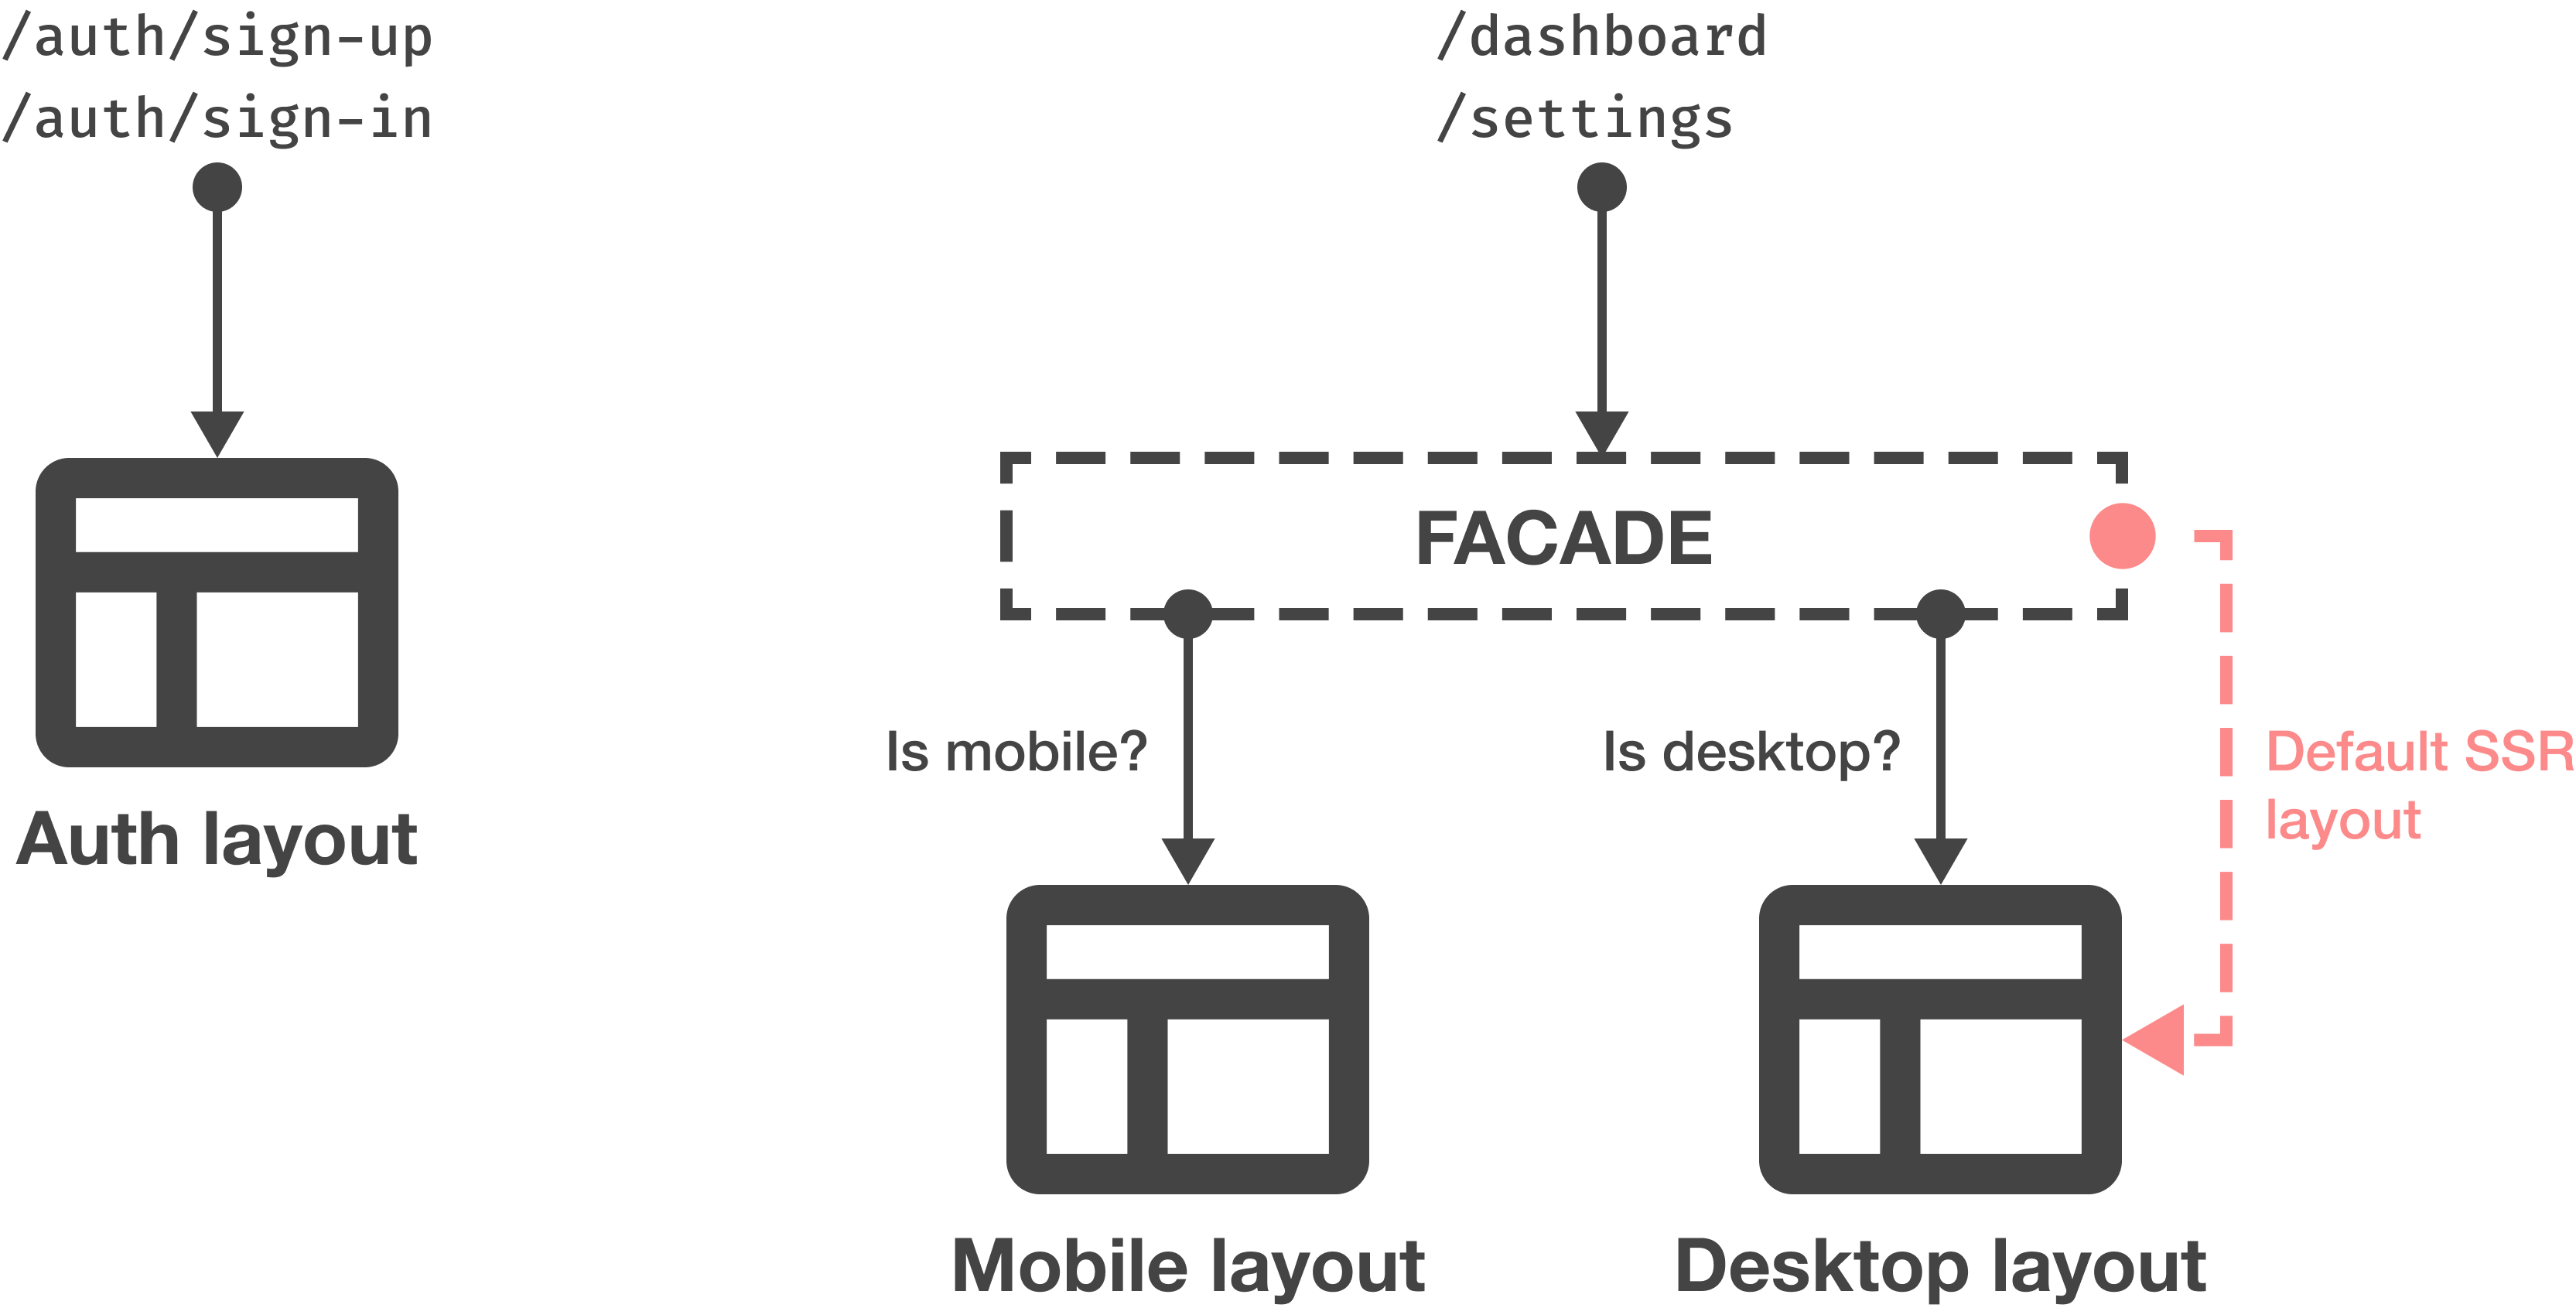
\includegraphics[width=0.75\textwidth]{./assets/designs/layout-facade.png}
	\caption{Component facade diagram}
\end{figure}
When the user enters one of the authentication URLs, which are
\texttt{/auth/sign-up} or \texttt{/auth/sign-in}, the authentication layout will
render the mobile or desktop version, depending on the screen viewport detected.
\\
On the other hand, when the user enters one of the authenticated pages, since
the layout has to change drastically, there are some logic aspects that need to
be taken into account. Therefore, in order to avoid having to copy and paste this
logic to every authenticated page, such logic it is kept in a single component,
that will render one layout or the other. Moreover, new added pages will be able
to use the same layout without the need of adding any additional logic.
\subsubsection{Authentication layout}
Starting with the sign-up layout page, it is divided in two different parts: the
content and the footer.
\begin{figure}[H]
	\centering
	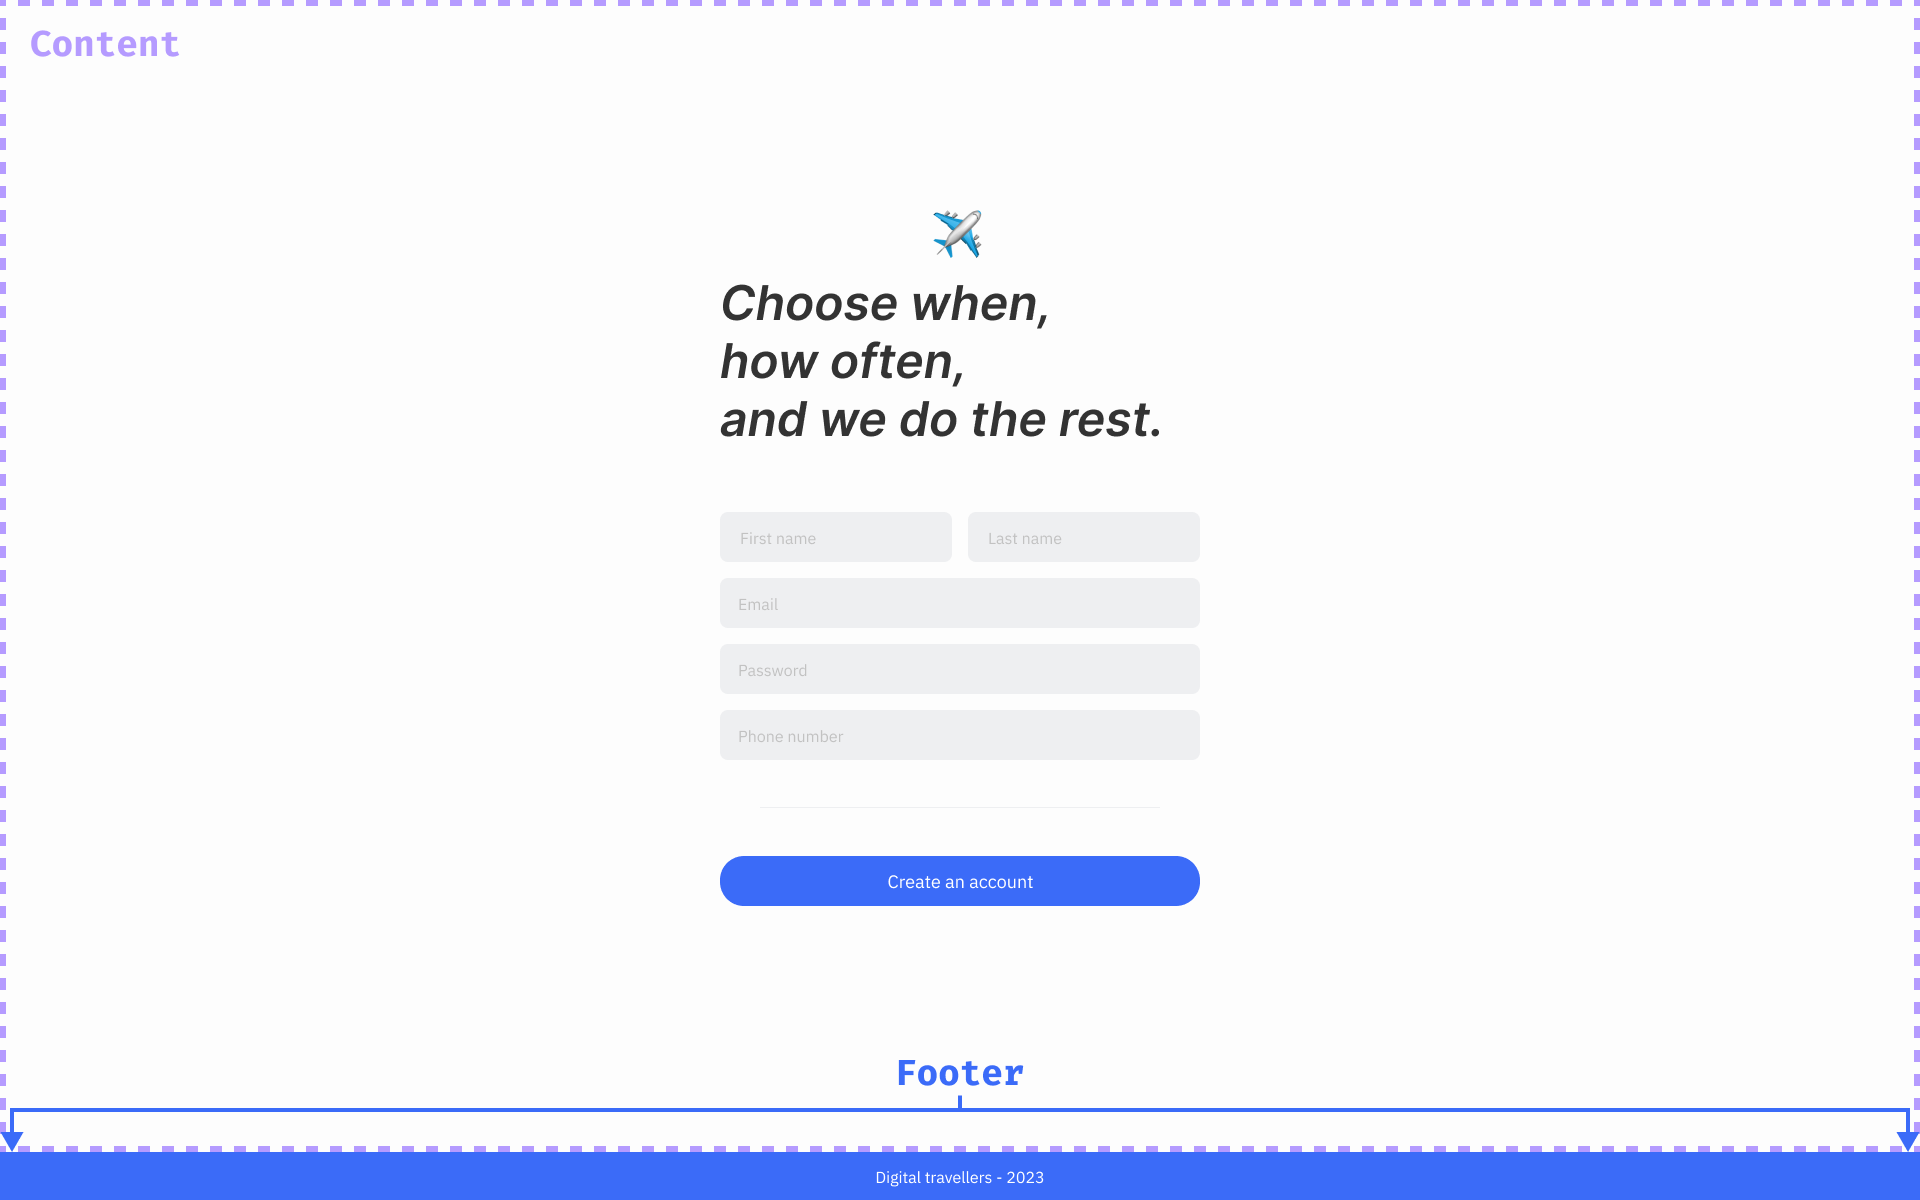
\includegraphics[width=\textwidth]{./assets/designs/sign-up-layout-web.png}
	\caption{Web version sign-up layout}
\end{figure}
The only difference with the mobile version is the colour of the footer. This
logic can be updated by using CSS media queries, as it will be faster than using
JavaScript. Furthermore, since the styles has been added using TailwindCSS,
media queries are even simpler.
\begin{figure}[H]
	\centering
	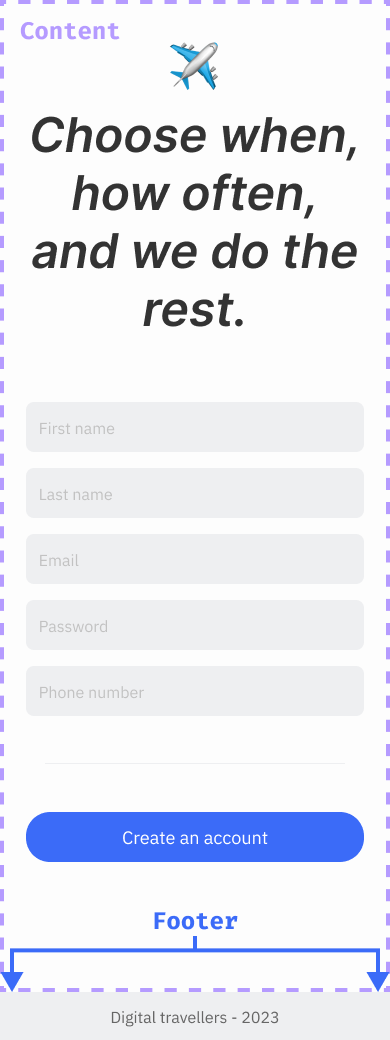
\includegraphics[width=0.25\textwidth]{./assets/designs/sign-up-layout-sm.png}
	\caption{Mobile version sign-up layout}
\end{figure}
\subsubsection{Authenticated layout}
The authenticated layout is slightly more complex than the authentication
layout. It is composed of the 4 following parts:
\begin{enumerate}[label = -]
	\item Green part (top-left rectangle) is a section to display the logo of the
	      application, in order to add branding material inside the application.
	\item The \textbf{navigation header}, which does not strictly contain
	      navigation elements, it displays information about the current page status.
	      In this case, it displays the dashboard title, as well as a message
	      underneath.
	\item The \textbf{sidebar}, which internally contains a sidebar menu. This
	      sidebar contains the navigation items and is going to display the current
	      page in which the user is. This last feature has been added during the
	      development, but was not contemplated in the initial designs.
	\item Finally, the \textbf{main content} which is the part that will be
	      constantly updated, when changing pages or via user interaction.
\end{enumerate}
Therefore, the developer will only need to take into account the changes inside
the \textbf{main content}, which, in the dashboard's case, involves having a
card and displaying the table with the alerts.
\\[8pt]
I also took the opportunity to mark with grey rectangles some of the components
that have already been defined and implemented, which in this case are the title
of the page and the subtitle. Moreover, the \textbf{sidebar menu} will also
contain typography items, which are components that have already been defined,
simplifying the implementation of the sidebar. It is worth mentioning that there
are other components such as the content button or the content title, that are
also already defined components.
\\[8pt]
Another point that has been taken into account has been the proper usage of
markup language. The following image illustrates the usage of the HTML
components:
\begin{figure}[H]
	\centering
	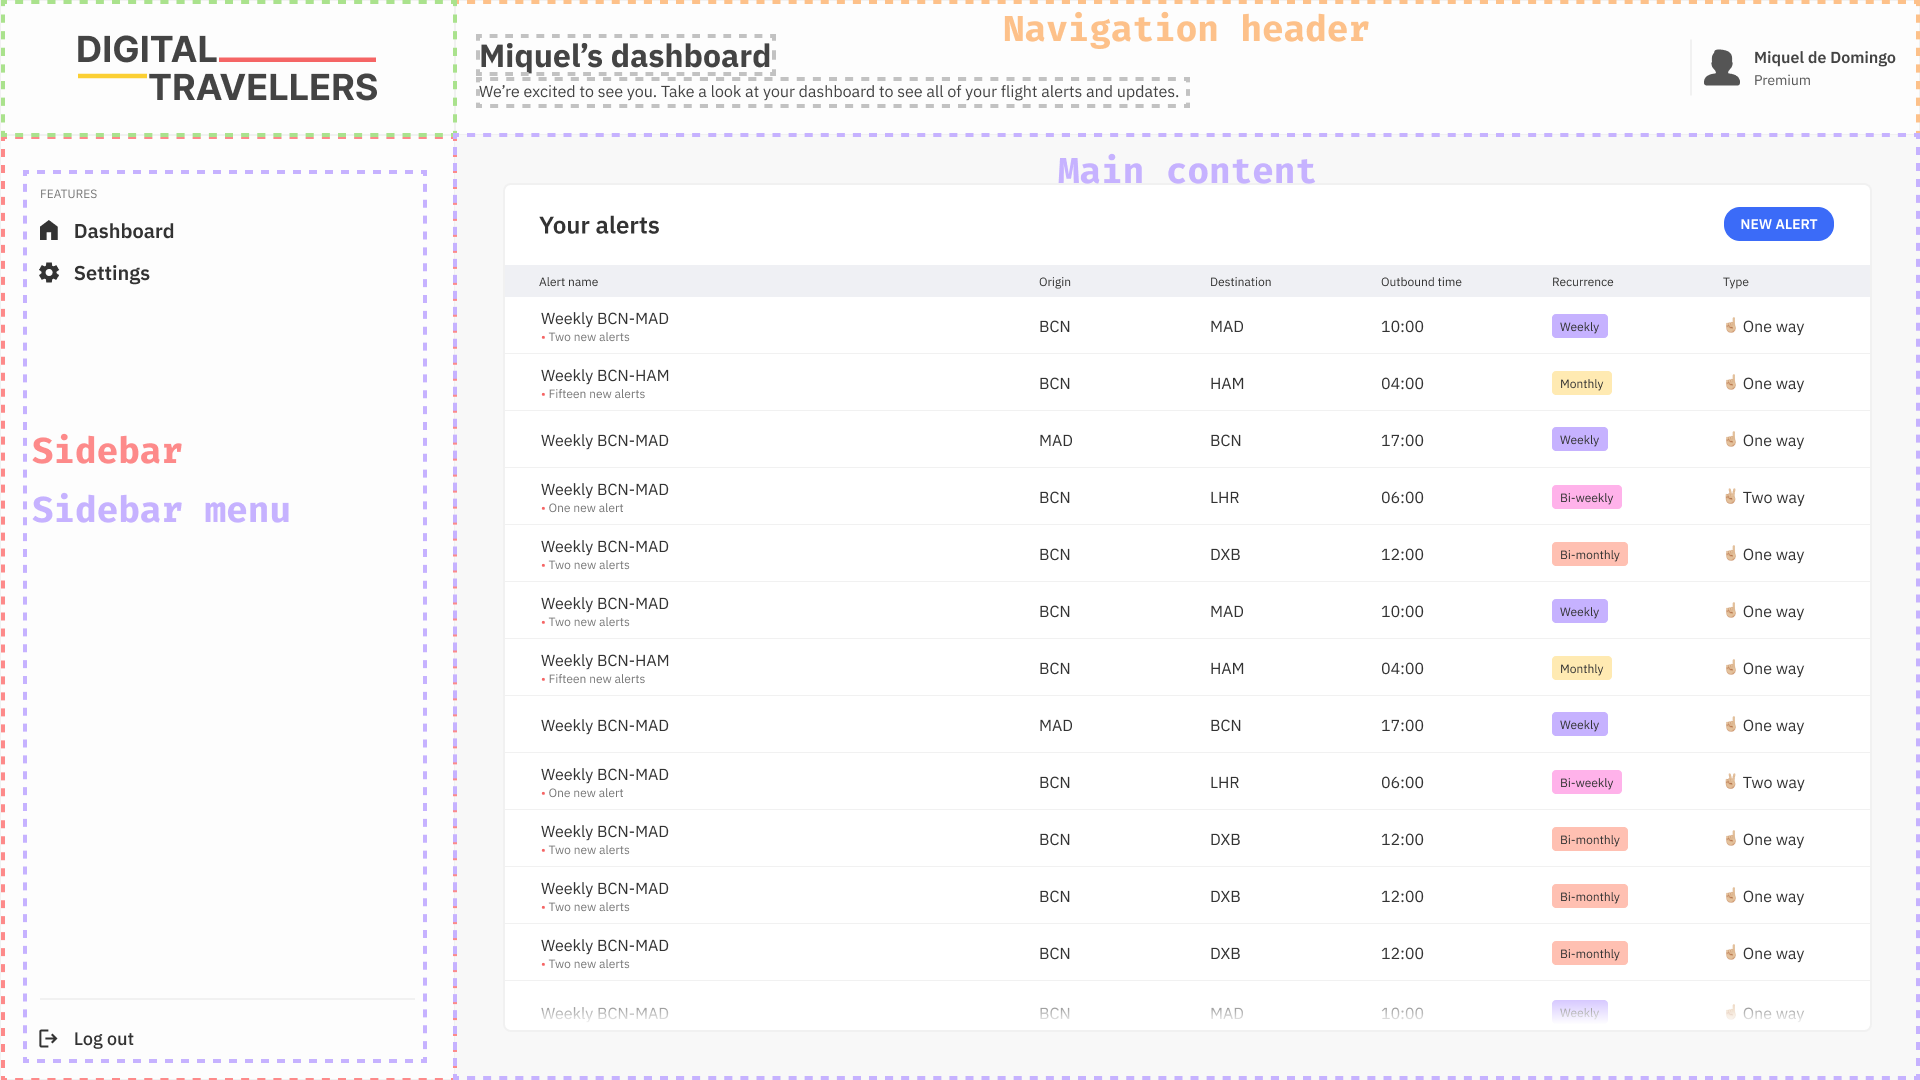
\includegraphics[width=\textwidth]{./assets/designs/dashboard-layout-web.png}
	\caption{Semantic HTML markup usage}
\end{figure}
Without taking into account the sizes, the layout is composed according to
expected markup. One could argue if an \texttt{article} should be used over the
\texttt{section}. However, according to the MDN documentation:
\begin{enumerate}[label = -]
	\item\textbf{Article}. \emph{The} \texttt{<article>} \emph{HTML element
		represents a self-contained composition in a document, page, application or
		site, which is intended to be independently distributable or
		reusable.} \cite{mdn-article}
	\item\textbf{Section}. \emph{The} \texttt{<section>} \emph{HTML element
		represents a generic standalone section of a document, which does not have a
		more specific semantic element to represent it.} \cite{mdn-section}
\end{enumerate}
Taking both definitions into account, the \texttt{section} component
semantically fits better than the \texttt{article} component.
\begin{figure}[H]
	\centering
	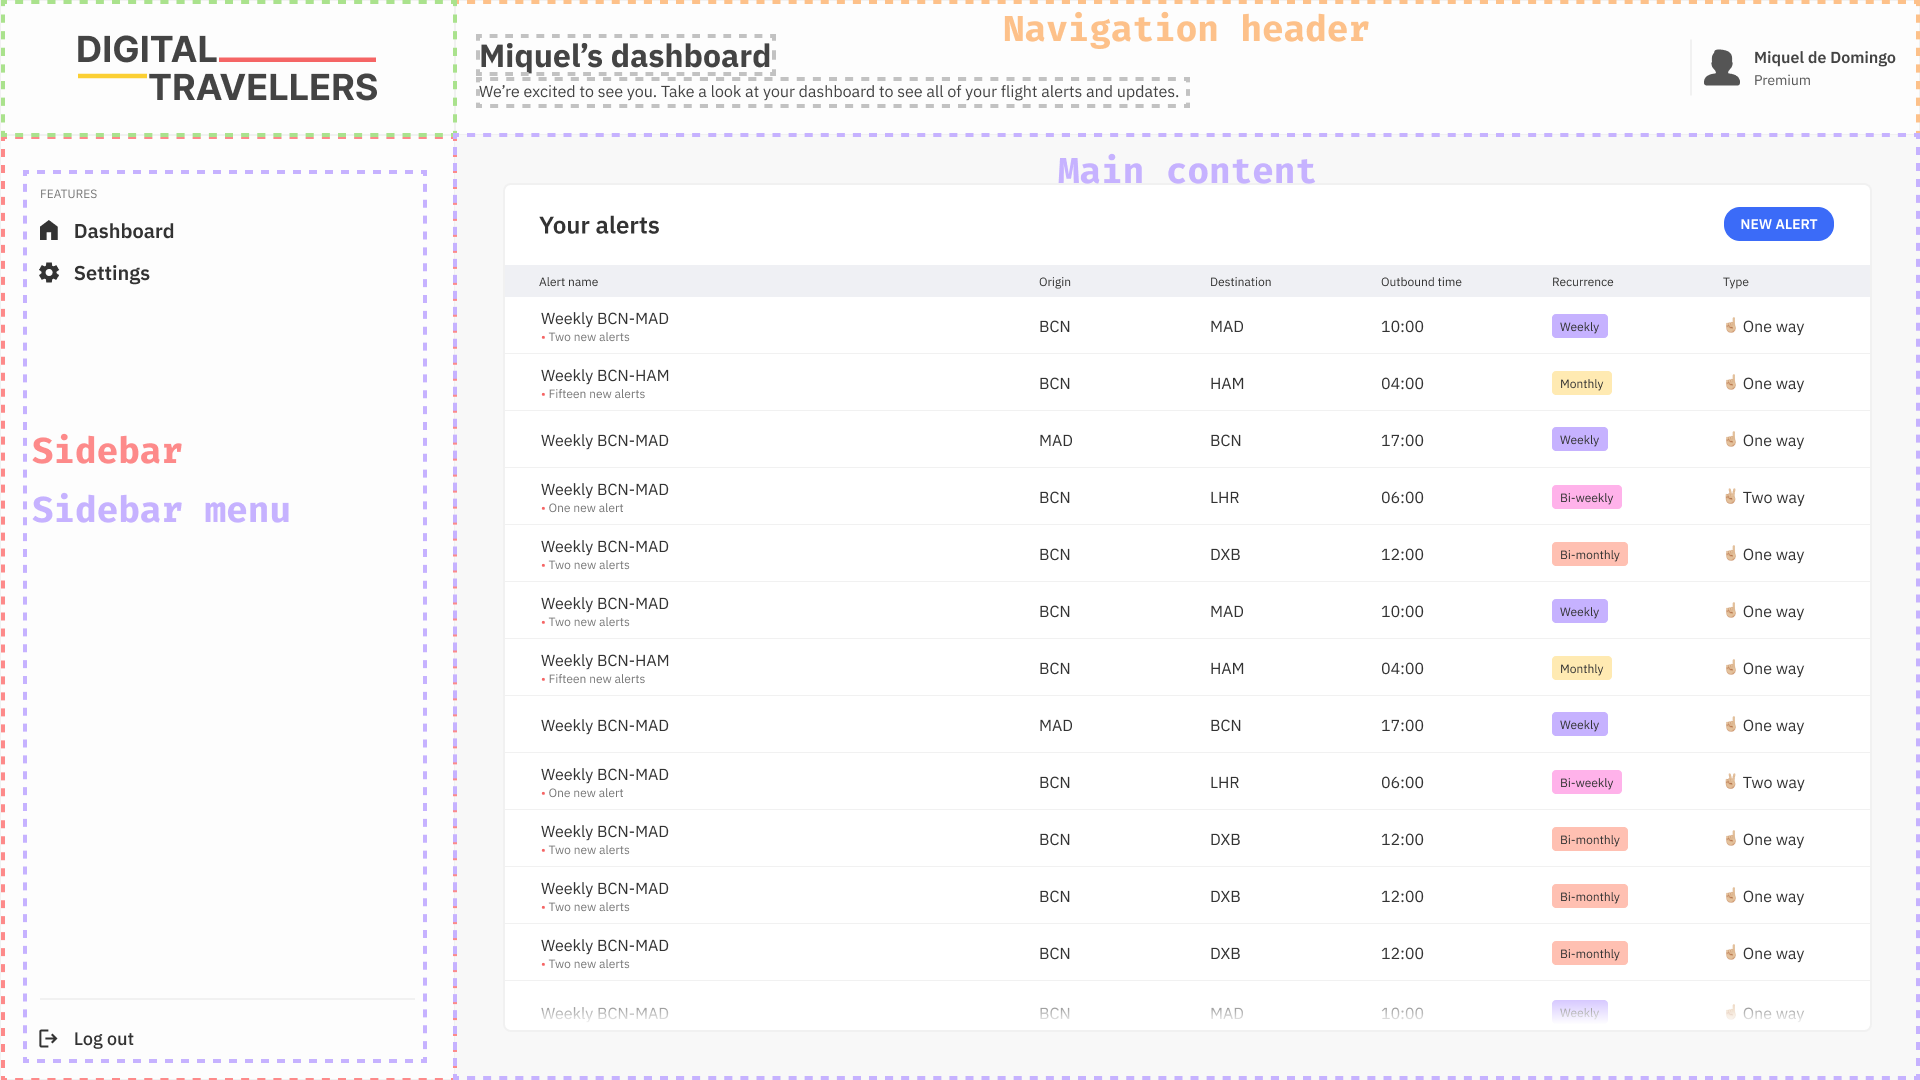
\includegraphics[width=\textwidth]{./assets/designs/dashboard-layout-web.png}
	\caption{Desktop version dashboard layout}
\end{figure}
Finally, the layout is compared with the mobile version layout. As can be seen,
the sidebar and branding element have been removed as they do not fit and do not
provide value for mobile users. However, the navigation header and content have
been retained. The HTML markup remains relevant, so the previous markup diagram
still applies.
\\[8pt]
However, the user still requires some form of navigation or sidebar. This
navigation has been hidden in the top-right button, which functions as a
hamburger menu. Initially, the idea was that clicking the cog button would
redirect the user to the settings page. However, this option did not account for
the addition of new pages, and implementing a hamburger menu that opens a
popover or full-screen overlay was deemed a better and more scalable solution.
\begin{figure}[H]
	\centering
	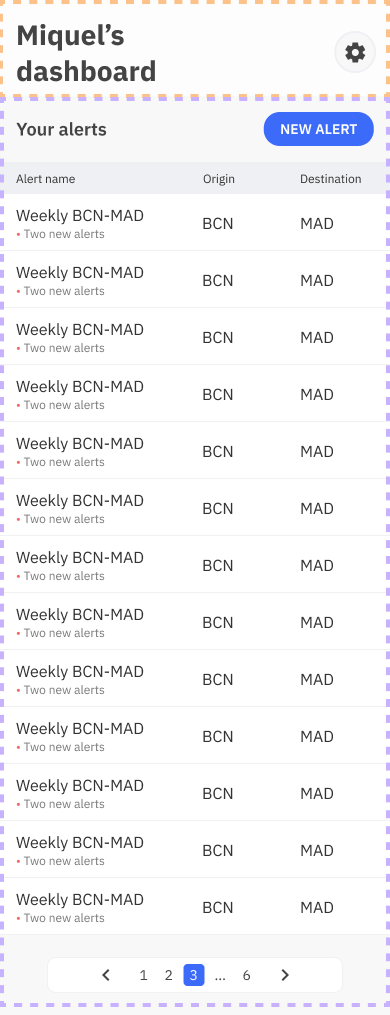
\includegraphics[width=0.25\textwidth]{./assets/designs/dashboard-layout-sm.png}
	\caption{Mobile version dashboard layout}
\end{figure}
\subsection{State management}
Finally, the last missing piece of the application is the state management of it.
State management is the process of maintaining the information of an application's
across multiple related data flows. In React, it is the process of managing and
synchronizing data within an application, and apply the changes to the user
interface accordingly.
\\[8pt]
React provides a built-in mechanism for state management named
\texttt{useState} (a hook). This hook allows functional or modern
components\footnote{Before React 16, components were class based.} to have their
own internal state. With the state definition and its updater function, React
handles the management of state changes and triggers re-renders when the state
is updated.
\\
However, as applications grow in complexity, the need for a most robust and
scalable state management solution is required. Though React provides a built-in
tool named \texttt{Context}, there are many other solutions that provide better
performance such as jotai \cite{jotai}, zudstand \cite{zudstand}, Recoil \cite{recoil}
or React Query \cite{react-query}\footnote{Currently rebranded as TanStack Query,
	though within the community it is still known as React Query.}.
\\[8pt]
Given that there are many possible state management solutions, the chosen
solution depends on various factors such as project size, complexity, or even
personal preferences. It is important to consider trade-offs between simplicity,
performance, development efficiency, and current maintenance
status\footnote{This point is sometimes overseen by developers. If third-party
	library has to play such an important role in an application, it is important
	that this library is currently maintained and up-to-date with current
	technologies.}.
\\[8pt]
For the current application, React Query (or TanStack Query) has been preferred
since not only provides a state management solution, but also a data fetching
system.
\subsubsection{React Query}
React query provides a declarative and intuitive approach to managing
asynchronous data, making it easier to interact with the server, while also
providing caching utilities, and state synchronization.
\\[8pt]
At its core, React Query revolves around the concept of queries and mutations:
\begin{enumerate}[label = -]
	\item Queries are used to fetch data from an API.
	\item Mutations are used to handle data updates, such as creating, editing
	      or deleting resources.
\end{enumerate}
When a query is executed, React Query will take care of the lifecycle of the
data fetching, by keeping track of the process. Under the hood, it manages data
caching and background re-fetching, ensuring that data remains up to date,
without unnecessary network requests. The caching system is flexible and
efficient enough to allow developers to control how data is stored and
invalidated.
\\
One of the most used features from React Query is the returned status of the
query or mutation execution. For each hook run, it is possible to know its
status:
\begin{enumerate}[label = -]
	\item\texttt{Loading}. Property that allows you to know if the query is
	being fetched. In this case, RQ\footnote{React Query} has checked if there
	was data in the cache but has not found any.
	\item\texttt{Error}. If the query or mutation resulted in an error (i.e.
	backend returned non-successful response), the error will be stored in this
	property.
	\item\texttt{Success}. The query or mutation has received a response, without
	an error, and it is ready to display the data received if any.
	\item\texttt{Idle}. Queries are run by default on mounting the component.
	However, it is possible to skip the execution of it. If that is the case,
	the query is left on idle, until the skip condition is false (so it can be
	executed).
\end{enumerate}
React Query mutations are a key aspect of the React Query library that enable
easy handling of data updates, such as creating, updating, and deleting
resources. Mutations provide a declarative way to interact with the server and
manage the state of the application based on these updates. React Query's
\texttt{useMutation} hook allows components to initiate mutations and provides
functions to execute the mutation, handle success and error cases, and update
the cache accordingly. With mutations, developers can perform optimistic
updates, where the UI is instantly updated with the expected result before the
server responds, providing a seamless user experience. React Query also supports
various options for configuring mutations, such as defining custom update
functions, invalidating related queries after a mutation, and providing
optimistic response data.
\begin{figure}[H]
	\centering
	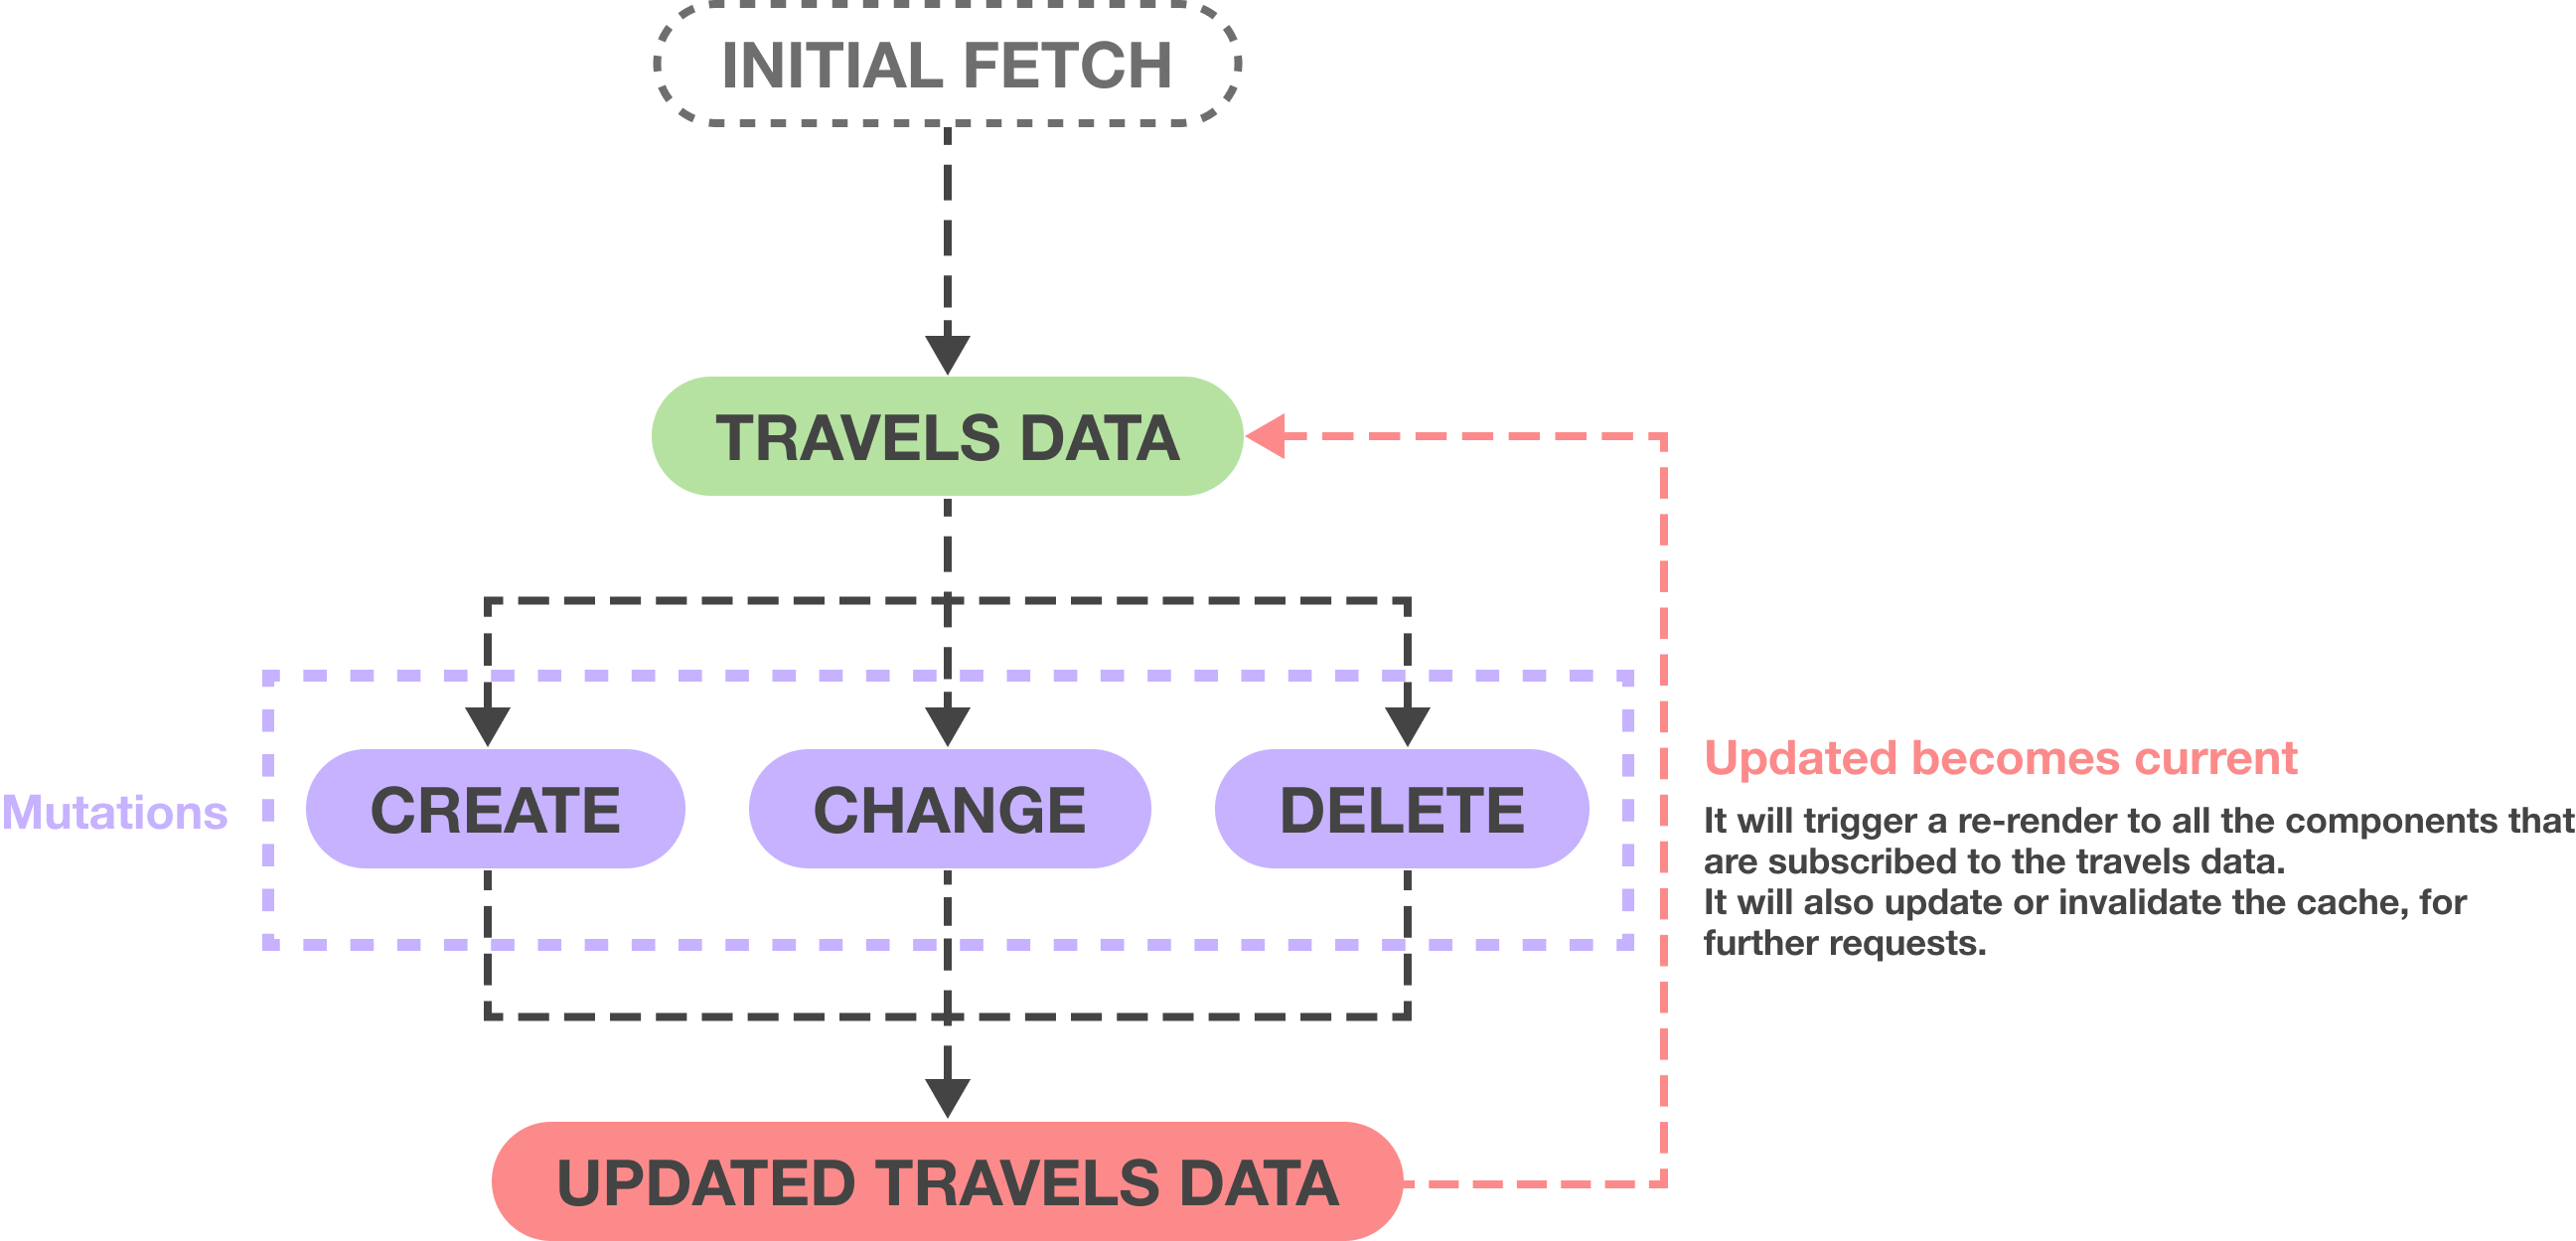
\includegraphics[width=\textwidth]{./assets/react-query-travels.png}
	\caption{React Query travels data flow}
\end{figure}
The picture above briefly illustrates how React Query interacts with the
travels' data. As it can be seen, an initial fetch is performed, which will load
the list of alerts in the cache and in the local state. Then, if by any chance
the user either creates, updates or deletes an alert, the previous state will
become invalid and will be updated accordingly. However, not all mutations must
invalidate some fetched data. For example, in order to authenticate the user,
mutations are also used, yet they do not invalidate any previously fetched data.
\\[8pt]
React Query helps with state management by providing a unified and consistent
approach to data management across the application. It abstracts away the
complexities of managing remote data and provides a single source of truth for
accessing and updating data. Components can easily subscribe to and interact
with the cached data using the provided hooks, reducing boilerplate code and
making state management more intuitive.
\\[8pt]
To sum up, all state management has been is being managed by React Query,
simplifying the frontend code, as there is no need for any state management
logic required, other than the React Query hooks.
\\
Since the user is not updated because the settings page has not been
implemented, there is no need to keep user state as part of the React Query
client. Alternatively, the React Context API has been used, since it is suitable
enough for our current logic.
\subsection{Integration over unit testing}
The topic of preferring integration to unit testing for the frontend
application has briefly been introduced in previous sections. However, a
justification is required and such is the goal of this section. There are
several reasons, and my own experience developing frontend react applications,
that have pushed me to prefer integration to unit testing.
\\[8pt]
First key factor, by applying hexagonal architecture, an effort was made to keep the
domain logic in a separate package, which has already been extensively unit
tested and integration tested. This ensures that the core functionality of the
application is thoroughly validated, reducing the need for duplicative unit
tests in the frontend components.
\\[8pt]
Another factor that has influenced this decision has been the usage of a tool
named \emph{Mock Service Worker} (MSW) alongside React Query, which has been
explained in the previous section. MSW allows the mocking of API requests and
responses, enabling comprehensive integration testing of data fetching and
management without the need for actual network calls or other complex mocking
set up. Furthermore, it allows the developers to simulate a semi-real
environment, as it provides utilities to simulate the delay between API calls,
while maintaining the integrity of the results. React Query, on the other hand,
provides a powerful data caching and synchronization mechanism, which simplifies
the testing of data-driven components that relied upon asynchronous data
fetching.
\\[8pt]
The presence of non-complex forms, such as the authentication ones, and complex
forms, such as the creation of a travel, emphasized the need for integration
testing. Forms often involve intricate interactions and validations that span
over multiple components and user or data flows. By focusing on integration
testing, it is possible to test the entire for workflow, including user
interactions, data submission, and error handling, ensuring a robust and
seamless user experience.
\\[8pt]
Additionally, the emphasis has been placed in testing user flows rather than
individual component integrity. Integration testing has allowed the simulation
of realistic user scenarios, such as the interaction with various components,
and validation of the overall application behaviour. This approach has provided
grater confidence in overall user experience and ensured that the application
functions as expected in a real-world usage.
\\[8pt]
It is also important to recognize that achieving high code coverage through unit
tests does not necessarily guarantee better code quality or a bug-free
application. Focusing solely on unit testing can sometimes lead to an excessive
focus on isolated component behaviour, overlooking potential issues that may
arise from the interactions between components or external dependencies.
Integration testing, on the other hand, helps uncover these potential
integration issues and ensures that the applications and components behave
correctly as a whole.
\\[8pt]
As a disadvantage, it is important to note that integration tests tend to
require more execution time, even though it should not be extremely high
(consider between 2 minutes to 10 minutes at most). In comparison, unit test
will run faster.
\\[8pt]
In conclusion, by prioritizing integration testing in the frontend part of the
application (excluding the domain and the shared UI library package), the
development team has been able to validate the user flows and data management.
The usage of tools like MSW and React Query, along with the consideration of
complex forms and user experience, have further supported the decision to favour
integration testing over unit testing. Ultimately, this approach has provided a
more comprehensive and reliable testing strategy for the application
\\[8pt]
As a last note for this section, there are some utilities such as helper
functions that have been unit tested, as in this case it has been considered
important to ensure the behaviour of them.
\section{CI/CD}
Last aspect to talk about regarding the implementation process, is the
continuous implementation and continuous development setup. Since the team
codebase is hosted in GitHub, the easiest tool to set up is GitHub Actions.
Furthermore, Nx's documentation has tutorials\cite{nx-github-actions} regarding
the implementation of the continuous integration in GitHub Actions.
\\[8pt]
In Nx, each project is configured with a set of commands tailored to its
specific type. For example, the \texttt{context} package includes commands such
as \texttt{lint}, \texttt{build} and \texttt{test}. The \texttt{lint} commands
checks for static errors in the package codebase, while \texttt{build} handles
bundling and generates the transpiled code. The \texttt{test} command executes
all the tests associated with the \texttt{context} package.
\\
One of the notable features of Nx is command parallelization, which allows
multiple commands to run concurrently, even within projects. This capability
significantly reduces the overall execution time in CI workers, improving its
efficiency. Furthermore, Nx Cloud offers the option to cache command output,
which means that if the package's codebase remains unchanged, Nx can rely on the
cached output, rather than re-executing the command, further optimizing
performance. Nonetheless, this feature has not been used as it is a paid
feature.
\\
Another standout features of Nx is its ability to identify updated packages. It
intelligently determines which packages have been modified and selectively runs
the associated commands only on those affected packages and their dependent
packages. This targeted approach reduces the complexity of the CI/CD
environment setup, and ensures that only necessary actions are performed, saving
time and resources.
\begin{figure}[H]
	\centering
	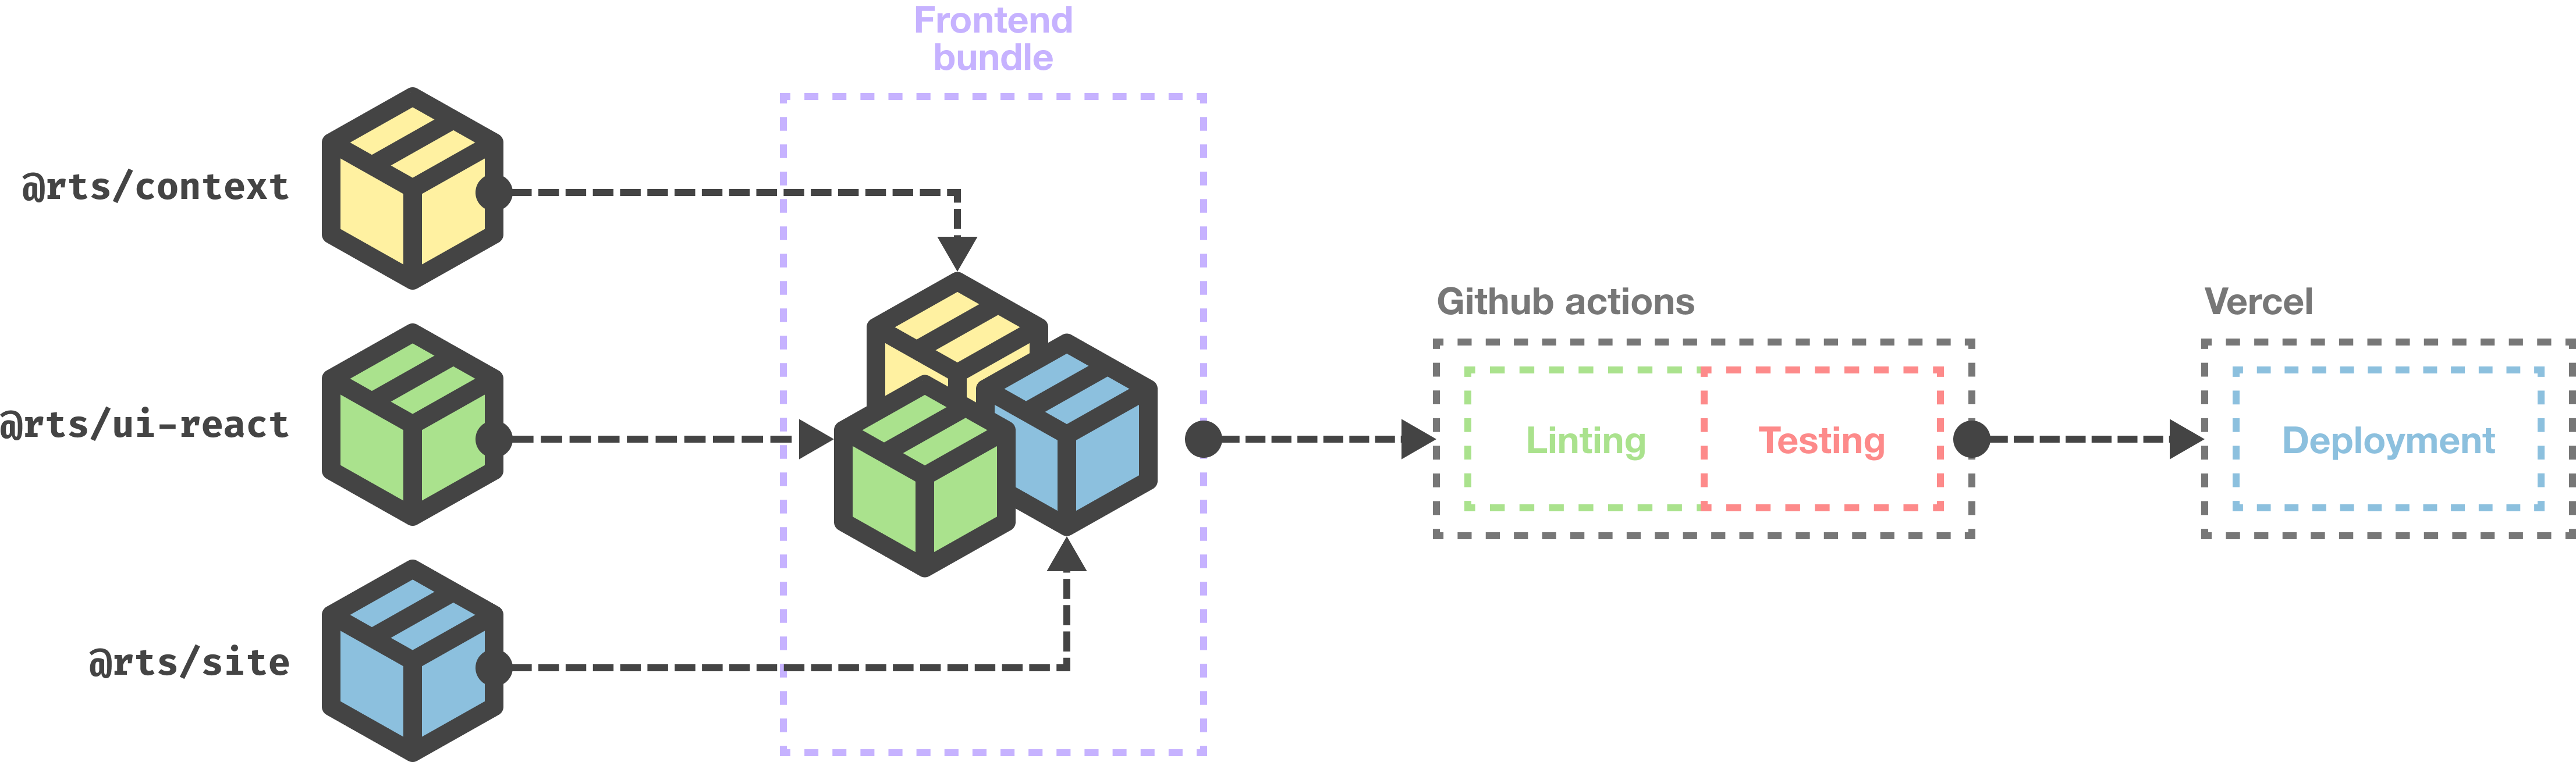
\includegraphics[width=\textwidth]{./assets/deployment.png}
	\caption{CI/CD flow}
\end{figure}
As it can be seen in the above diagram, the last step of the flow is the
deployment to Vercel. The Vercel option was chosen because of its simplicity. By
configuring certain aspects of the repository, the Vercel infrastructure it is
capable to identify and understand the codebase, and properly deploy the
application. Since Nx provides all build commands and utilities, there is no
need to configure anything extra, aside from setting the command to use.
\\
Vercel is an extremely powerful tool, however, due to the lack of time and
simple implementation, aside from the automated deployment on \texttt{main}
branch merge, nothing else has been used.
\section{Code structure}
As the final section of this chapter, the goal is to explain the code structure
of the various packages and the reasoning behind it.
\subsection{Context package}
The context package follows a modular organization, as recommended by hexagonal
architecture principles. It adheres to a layered architecture, with clear
separation between application, domain, and infrastructure layers
\begin{enumerate}[label = -]
	\item\texttt{src}. The source folder contains the source code of the project
	excluding the tests. It is divided following the hexagonal architecture
	principles. Some layers may include a \texttt{shared} submodule, which contains
	shared code within the different sub-modules.
	\begin{enumerate}[label = -]
		\item\texttt{app}. The \texttt{app} folder represents the application
		layout of the project. Inside, it is organized by submodules for
		different application implementation, such as the authentication
		(\texttt{auth}) and the travels (\texttt{travel}).
		\item\texttt{domain}. The directory represents the domain layer of the
		project. It is also divided in submodules, which should match the
		application ones.
		\item\texttt{infra}. The infrastructure directory represents the custom
		definition of the infrastructure layer. As explained in previous
		chapters, the infrastructure is divided in queries and queriers.
	\end{enumerate}
	\item\texttt{test}. The test package contains the unit and integration tests
	for the context package. Internally, it clones the same structure as the
	\texttt{src} folder.
	\begin{enumerate}[label = -]
		\item\texttt{app}. The \texttt{app} directory contains the tests for the
		application layer, mirroring the structure in \texttt{src/app}
		directory.
		\item\texttt{domain}. The \texttt{domain} directory includes the test
		files for the domain layer, mirroring the structure in
		\texttt{src/domain}. It also includes \texttt{mothers} directories,
		which contain randomized data generation for the different entities.
		\item\texttt{infra}. The directory includes the test files for the
		infrastructure layer, also mirroring the structure in
		\texttt{src/infra}. It also contains the setup and handlers for the
		MSW\footnote{Mock service worker.} that it is used for integration
		tests.
		\item\texttt{util}. Contains shared utilities for the testing folder.
	\end{enumerate}
\end{enumerate}
\subsection{UI React library}
The UI react library follows a standard \emph{folder per component} or related
components. Inside each folder, it can be found:
\begin{enumerate}[label = -]
	\item The implementation of the component or various components. One component
	      per file.
	\item A \texttt{spec} file with the tests for the component.
	\item The \texttt{stories} file type that contains the implementation of the
	      component to be visualized in the Storybook application.
	\item Possibly a \texttt{d} or declaration file, for TypeScript types. If
	      there are few types, this file is not contained.
\end{enumerate}
This \emph{folder per component} is extremely useful for libraries, because as
the library grow, it can simplify the code splitting and tree shaking. This
benefits will reduce the bundled code size, reducing the amount of code sent to
the user's browser.
\subsection{Site application}
The site application is divided in the following folders:
\begin{enumerate}[label = -]
	\item\texttt{components}. This folder contains reusable components used
	throughout the application. It also follows the \emph{folder per component}
	in order to reduce complexity and keep the codebase organized. As a personal
	preference, I prefer organization through folders rather than files.
	\item\texttt{config}. This folder holds configurations files for the
	application, as well as global constants such as the route paths of the app.
	The goal is to have a unique source of truth for such topics.
	\item\texttt{domain}. The directory represents the domain-specific code for
	the different pages. In this case, it has been preferred to keep a
	domain per specific route. This allows the domain to keep escalating
	without issues.
	\item\texttt{hooks}. This directory contains custom React hooks used
	within the application. It also contains the abstraction of the React
	Query hooks logic into other hooks.
	\item\texttt{layouts}. This directory houses the layout components used
	for different pages of the application.
	\item\texttt{msw}. This directory contains the implementation of the MSW used
	for local development and testing.
	\item\texttt{pages}. The \texttt{pages} directory holds the Next.js page
	components that define the routes and rendering logic for different URLs
	of the application.
	\item\texttt{public}. This directory is used for static assets that are served
	publicly, such as images or fonts.
	\item\texttt{styles}. This directory contains global CSS styles, as well as a
	reference for the TailwindCSS utilities.
	\item\texttt{test}. Even though each element contains the text in the same
	file level, the \texttt{test} directory contains shared utils for the tests.
\end{enumerate}
Overall, the folder structure is Next.js standard, with some customizations,
since React does not provide an official or recommended way of structuring the
code.
\end{document}
